\documentclass[12pt]{aghdpl}
% \documentclass[en,11pt]{aghdpl}  % praca w języku angielskim
\usepackage[polish]{babel}
%\usepackage[english]{babel}
\usepackage[utf8]{inputenc}
\usepackage[hidelinks]{hyperref}

% dodatkowe pakiety
\usepackage{enumerate}
\usepackage{listings}
\usepackage{setspace}
\usepackage{nameref}
\usepackage{upquote}
\usepackage{longtable}
%\usepackage{lmodern}
\usepackage{amsmath}
\usepackage{fixltx2e} % provides \textsubscript
% use upquote if available, for straight quotes in verbatim environments
\IfFileExists{upquote.sty}{\usepackage{upquote}}{}
% use microtype if available
\IfFileExists{microtype.sty}{%
\usepackage{microtype}
\UseMicrotypeSet[protrusion]{basicmath} % disable protrusion for tt fonts
}{}
\usepackage{longtable,booktabs}
\urlstyle{same}  % don't use monospace font for urls
\setlength{\parindent}{0pt}
\setlength{\parskip}{6pt plus 2pt minus 1pt}
\setlength{\emergencystretch}{3em}  % prevent overfull lines

\lstloadlanguages{TeX,Bash}

\lstset{
  literate={ą}{{\k{a}}}1
           {ć}{{\'c}}1
           {ę}{{\k{e}}}1
           {ó}{{\'o}}1
           {ń}{{\'n}}1
           {ł}{{\l{}}}1
           {ś}{{\'s}}1
           {ź}{{\'z}}1
           {ż}{{\.z}}1
           {Ą}{{\k{A}}}1
           {Ć}{{\'C}}1
           {Ę}{{\k{E}}}1
           {Ó}{{\'O}}1
           {Ń}{{\'N}}1
           {Ł}{{\L{}}}1
           {Ś}{{\'S}}1
           {Ź}{{\'Z}}1
           {Ż}{{\.Z}}1
}

\definecolor{mygray}{rgb}{0.5,0.5,0.5}
\lstdefinestyle{console}{
  commentstyle=\color{mygray},
  basicstyle=\ttfamily\footnotesize,
  tabsize=2,
  rulecolor=,
  basicstyle=\scriptsize,
  upquote=true,
  aboveskip={1.5\baselineskip},
  columns=fixed,
  showstringspaces=false,
  extendedchars=true,
  breaklines=true,
  prebreak = \raisebox{0ex}[0ex][0ex]{\ensuremath{\hookleftarrow}},
  frame=single,
  showtabs=false,
  showspaces=false,
  escapechar=\\,
  showstringspaces=false,
  identifierstyle=\ttfamily
}

%---------------------------------------------------------------------------

\author{Łukasz Opioła, Beata Skiba}
\shortauthor{Ł. Opioła, B.Skiba}

\titlePL{Dokumentacja projektowa: "Analiza przyczyn wypadków drogowych"}
\titleEN{}

\shorttitlePL{Przyczyny wypadków drogowych} 
\shorttitleEN{}

\thesistype{Zaawansowane Techniki Integracji Systemów}

\degreeprogramme{Informatyka}

\date{2015}

\department{Katedra Informatyki}

\faculty{Wydział Informatyki, Elektroniki i Telekomunikacji}


\setlength{\cftsecnumwidth}{10mm}

%---------------------------------------------------------------------------

\begin{document}

\titlepages

\tableofcontents

\chapter{Temat i cel projektu}
\label{chap:cel}
\section{Temat projektu}\label{temat-projektu}

Tematem projektu jest integracja różnych źródeł danych opisujących
przyczyny wypadków drogowych. Temat obejmuje identyfikację
reprezentatywnych źródeł i zebranie z nich danych, sprowadzenie ich do
wspólnej reprezentacji a następnie poddanie tak przetworzonych danych
wieloprzekrojowej analizie.

\section{Cel projektu}\label{cel-projektu}

Głównym celem projektu jest analiza danych na temat wypadków drogowych
pod kątem prawdopodobnych przyczyn.

Można wyróżnić kilka pośrednich celów, których realizacja będzie
konieczna w ramach projektu. Pierwszym z nich jest zgromadzenie danych
na temat wypadków drogowych, pochodzących z reprezentatywnych źródeł.
Obszarami, na których będziemy chcieli się skupić są Polska, Europa
Zachodnia, USA i Kanada. Celem naszym jest znalezienie danych godnych
zaufania, możliwie pełnych i obszernych oraz analiza informacji, jakich
te dane nam dostarczają. Aby umożliwić dalszą pracę z danymi
pochodzącymi z różnych źródeł, konieczne będzie sprowadzenie ich do
wspólnej reprezentacji danych, pozwalającej na dalszą analizę.

Kolejnym celem stawianym w projekcie jest umożliwienie wnioskowania o
przyczynach wypadków. Dane o przyczynach mogą być dostępne w danych
bezpośrednio, w przeciwnym razie konieczna będzie identyfikacja i
selekcja kryteriów, pozwalających na przeprowadzenie wnioskowania w tym
zakresie.

Ostatecznie celem projektu będzie przeprowadzenie analiz danych na wielu
płaszczyznach z wykorzystaniem określonych wcześniej kryteriów. Pozwoli
to zarówno na identyfikację możliwych przyczyn poszczególnych wypadków
jak i wyciągnięcie wniosków co do ogólnych przyczyn wypadków i
okoliczności zwiększających ryzyko ich wystąpienia.


\chapter{Plan pracy}
\label{chap:plan}
\section{Zadania projektowe i plan
pracy}\label{zadania-projektowe-i-plan-pracy}

\textbf{Zadanie:} \textbf{Zebranie danych} \textbf{Skrótowa nazwa:}
Zebranie danych\\\textbf{Czas realizacji:} 16.03 - 30.03\\\textbf{Opis:}
Identyfikacja i ocena dostępnych źródeł danych, wstępna analiza ich
przydatności i zawartości.\\\textbf{Produkty:} Artefaktem
potwierdzającym ukończenie zadania i zawierającym rezultaty
przeprowadzonych działań będzie dokument ``Analiza źródeł danych''

\textbf{Zadanie:} \textbf{Wybór atrybutów} \textbf{Skrótowa nazwa:}
Wybór atrybutów\\\textbf{Czas realizacji:} 30.03 - 13.04\\\textbf{Opis:}
Dogłębna analiza danych zawartych w źródłach i wybór kryteriów przyszłej
analizy oraz selekcja tych atrybutów ze źródeł, które będą konieczne do
realizacji celów projektowych.\\\textbf{Produkty:} Artefaktem z tego
zadania będzie dokument ``Kryteria analizy''

\textbf{Zadanie:} \textbf{Opracowanie wspólnego formatu danych i
schematu bazy}\\\textbf{Skrótowa nazwa:} Wspólny format\\\textbf{Czas
realizacji:} 06.04 - 20.04\\\textbf{Opis:} Stworzenie zgodnie z dokonaną
wcześniej selekcją atrybutów wspólnego formatu danych. Obejmuje zarówno
ujednolicenie formatu danych (np. data, sposób oznaczenia miejsca
wypadku) jak i semantyki (np. obranie wspólnych określeń na warunki
atmosferyczne panujące w momencie wypadku).\\\textbf{Produkty:} W
związku z tym zadaniem powstaną następujące artefakty: dokument
``Projekt bazy danych'' zawierający opis formatu i semantyki danych oraz
schemat bazy danych.

\textbf{Zadanie:} \textbf{Integracja danych i zapis do
bazy}\\\textbf{Skrótowa nazwa:} Integracja\\\textbf{Czas realizacji:}
13.04 - 04.05\\\textbf{Opis:} Ekstrakcja danych ze źródeł, transformacja
do wspólnego formatu i załadowanie do bazy danych. Obejmuje utworzenie
skryptów parsujących i konwertujących na wspólny format i wspólną
semantykę.\\\textbf{Produkty:} Produktami tego zadania będą skrypty oraz
uzupełniona baza danych.

\textbf{Zadanie:} \textbf{Statystyczna analiza danych}\\\textbf{Skrótowa
nazwa:} Analiza statystyczna\\\textbf{Czas realizacji:} 04.05 -
25.05\\\textbf{Opis:} Statystyczna analiza danych w celu wyłonienia
możliwych przyczyn wypadku, zgodna z określonymi wcześniej
kryteriami.\\\textbf{Produkty:} Realizacja tego zadania przejawi się w
następujących produktach: skrypty przeprowadzające analizy, wykresy
obrazujące przeprowadzone analizy, dokument ``Raport z analiz'', który
będzie tworzony stopniowo, być może jako zbiór mniejszych dokumentów
wraz z przeprowadzaniem kolejnych analiz oraz dokument ``Wnioski z
analiz'', który będzie opisywał wnioski na temat przyczyn wypadków
drogowych wyciągnięte na podstawie przeprowadzonych analiz.

\textbf{Zadanie:} \textbf{Zaawansowana analiza danych}\\\textbf{Skrótowa
nazwa:} Zaawansowana analiza\\\textbf{Czas realizacji:} 18.05 -
8.06\\\textbf{Opis:} Zaawansowana analiza danych w celu wyłonienia
możliwych przyczyn wypadku, korzystająca z mechanizmów takich jak
klasteryzacja czy wyszukiwanie wzorców częstych.\\\textbf{Produkty:}
Realizacja tego zadania przejawi się w następujących produktach: skrypty
przeprowadzające analizy, wykresy obrazujące przeprowadzone analizy,
dalsze części dokumentu ``Raport z analiz'', oraz dalsze części
dokumentu ``Wnioski z analiz'' (patrz zadanie Statystyczna analiza
danych).

\section{Wykres Gantta}\label{wykres-gantta}

Opisane powyżej zadania zostały przedstawione na wykresie Gantta,
zgodnie z przewidywanymi terminami ich wykonywania.

\begin{figure}[htbp]
\centering
\centerline{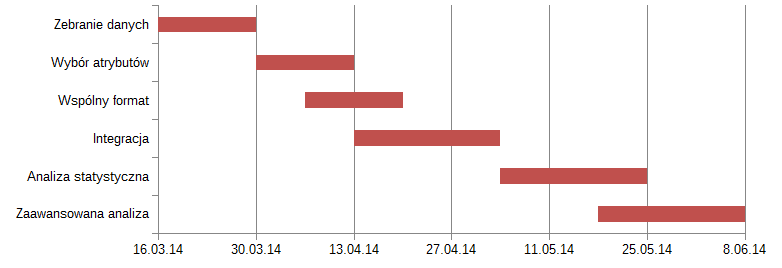
\includegraphics[width=0.9\textwidth]{images/gantt.png}}
\caption{Diagram Gantta}
\end{figure}

\section{Ryzyko w projekcie}\label{ryzyko-w-projekcie}

Prawdopodobieństwo wystąpienia oraz wpływ na projekt podane w skali 1-5

\textbf{Ryzyko:} Problem z uzyskaniem części danych\\\textbf{Opis:}
Otrzymanie danych z POBR jest uzależnione od fizycznej osoby, która musi
przydzielić możliwość pełnego dostępu do danych po wcześniejszym
otrzymaniu stosownego pisma. Procedura taka może za długo trwać i nie
zdążymy uwzględnić tych danych w projekcie.\\\textbf{Prawdopodobieństwo
wystąpienia:} 4\\\textbf{Wpływ na projekt:} 2\\\textbf{Rozwiązanie:}
Praca z danymi dostępnymi i uwzględnienie niedostępnych danych w postaci
statystyk

\textbf{Ryzyko:} Problem z ustaleniem wspólnego formatu
danych\\\textbf{Opis:} Dane, z których korzystamy, pochodzą z bardzo
różnych źródeł, mają różną semantykę i format. Może się okazać niezwykle
trudne stworzenie wspólnego formatu danych dla tych źródeł, które
jednocześnie będzie maksymalnie wykorzystywał dane w nich
dostępne\\\textbf{Prawdopodobieństwo wystąpienia:} 4\\\textbf{Wpływ na
projekt:} 4\\\textbf{Rozwiązanie:} W razie konieczności zawężenie
wspólnego formatu danych i w konsekwencji utrata części danych z
niektórych źródeł

\textbf{Ryzyko:} Duża ilość brakujących danych\\\textbf{Opis:} Wiele
przydatnych informacji może brakować dla części danych. Część ta może
się okazać bardzo duża\\\textbf{Prawdopodobieństwo wystąpienia:}
3\\\textbf{Wpływ na projekt:} 2\\\textbf{Rozwiązanie:} Problem
brakujących danych jest trudny do zwalczenia, gdyż nie ma możliwości
uzupełnienia ich wszystkich, należy więc w taki sposób zaprojektować
analizy aby uwzględnić możliwość braku niektórych danych.

\textbf{Ryzyko:} Duża ilość danych\\\textbf{Opis:} Źródła danych, z
którymi będziemy pracować w projekcie zawierają dużo
danych.\\\textbf{Prawdopodobieństwo wystąpienia:} 4\\\textbf{Wpływ na
projekt:} 2\\\textbf{Rozwiązanie:} Duża ilość danych jest z jednej
strony dobra gdyż pozwala stwierdzić reprezentatywność analiz i rozważyć
wiele przypadków, może być jednak kłopotliwa w przeprowadzaniu analiz.
Należy dobrze zaprojektować bazę danych i ograniczyć się do
przechowywania tych atrybutów, które będą naprawdę przydatne w analizie.
Analizy musza brać pod uwagę ilość danych i np. ograniczać się do
analizowania w danym momencie danych z jednego roku.


\chapter{Analiza źródeł danych}
\label{chap:analiza-zrodel}
\subsubsection{Cel dokumentu}\label{cel-dokumentu}

Niniejszy dokument ma na celu podsumowanie informacji na temat źródeł
danych, które będziemy mogli wykorzystać w projekcie. Charakterystyka
dokumentów obejmuje zakres danych, możliwe problemy z ich otrzymaniem i
wykorzystaniem a także zawartość danych - informacje o wypadkach, jakie
można znaleźć w opisywanych danych. Dokument zawiera również wstępną
definicję kryteriów, w ramach których będziemy analizować przyczyny
wypadków drogowych, z uwzględnieniem informacji o źródłach.

\section{Przegląd źródeł danych}\label{przeglad-zrode-danych}

Głównymi obszarami zainteresowania przy szukaniu źródeł danych były:
Polska, Europa Zachodnia, USA, Kanada

\begin{enumerate}
\item
  Polska

  \begin{itemize}
  \item
    Polskie Obserwatorium Bezpieczeństwa Ruchu Drogowego (POBR)

    \begin{itemize}
    \item
      \url{http://www.obserwatoriumbrd.pl/pl/}\\
    \item
      System składa się z dwóch części: hurtowni danych i portalu
      informacyjnego z interaktywną mapą do przeglądania danych z
      hurtowni.\\
    \item
      Dostęp jest ograniczony - bez rejestracji możliwy jedynie dostęp
      do wersji demo interaktywnej mapy oraz części zbiorczych
      statystyk.\\
    \item
      Studenci, dziennikarze, przedstawiciele społeczności lokalnych
      mogą uzyskać czasowy dostęp do pełnej bazy danych, po uprzednim
      pisemnym potwierdzeniu, że dane potrzebne będą do przygotowywanych
      opracowań.\\
    \item
      Z informacji na stronie wynika, że dane powinny być rzetelne i
      pełne.\\
    \item
      Kroki konieczne do otrzymania pełnego dostępu można znaleźć
      {[}tutaj{]}.(\url{http://www.obserwatoriumbrd.pl/pl/rejestracja/zasady_udostepniania})\\
    \item
      Wnioskując po wersji demo mapy interaktywnej, w hurtowni danych
      dostępne powinny być przynajmniej następujące informacje na temat
      wypadków:

      \begin{itemize}
      \item
        miejsce\\
      \item
        czas\\
      \item
        droga (numer, rodzaj)\\
      \item
        obszar zabudowany/niezabudowany\\
      \item
        informacje o uczestnikach i ofiarach wypadku

        \begin{itemize}
        \itemsep-14pt\parskip0pt\parsep0pt
        \item
          wiek\\
        \item
          płeć\\
        \item
          pojazd\\
        \item
          obrażenia\\
        \item
          ``ciężkość'' wypadku (śmiertelny, cięzki, lekki)\\
        \end{itemize}
      \item
        obecność alkoholu u sprawcy\\
      \item
        nadmierna prędkość\\
      \end{itemize}
    \end{itemize}
  \end{itemize}
\item
  Europa Zachodnia

  \begin{itemize}
  \item
    CARE

    \begin{itemize}
    \itemsep-14pt\parskip0pt\parsep0pt
    \item
      \url{http://ec.europa.eu/idabc/en/document/2281/5926.html} ,
      \url{http://ec.europa.eu/transport/road_safety/specialist/statistics/index_en.htm}\\
    \item
      Zawiera dane dostarczane przez odpowiednie instytucje ze
      wszystkich krajów Unii Europejskiej w postaci przetworzonej do
      wspólnego formatu\\
    \item
      Dostęp bezpośrednio do bazy niestety nie jest możliwy, dla
      wiadomości publicznej dostępne są tylko wybrane zbiorcze
      statystyki\\
    \end{itemize}
  \item
    Wielka Brytania

    \begin{itemize}
    \item
      \url{http://data.gov.uk/dataset/road-accidents-safety-data}\\
    \item
      Dane z wypadków na drogach publicznych, zgłoszonych na policję i
      odnotowanych przy wykorzystaniu formularza STATS19.\\
    \item
      Dane dostępne dla lat 1979 - 2013\\
    \item
      Dane obejmują m.in.:

      \begin{itemize}
      \itemsep-14pt\parskip0pt\parsep0pt
      \item
        okoliczności wypadku\\
      \item
        typy pojazdów (marka i model)\\
      \item
        dane o ofiarach\\
      \item
        informacje o poziomie alkoholu w wydychanym powietrzu\\
      \end{itemize}
    \end{itemize}
  \item
    Belgia-Flandria

    \begin{itemize}
    \itemsep-14pt\parskip0pt\parsep0pt
    \item
      \url{http://fimi.ua.ac.be/data/}\\
    \item
      Dane zebrane przez National Institute of Statistics (NIS)\\
    \item
      Obejmują lata 1991 - 2013 i tylko jeden region. Wydaje się, że
      jest to zbyt mocne ograniczenie.
    \end{itemize}
  \end{itemize}
\item
  USA i Kanada

  \begin{itemize}
  \item
    NHTSA: National Automotive Sampling System (NASS) - Crashworthiness
    Data System (CDS)

    \begin{itemize}
    \item
      \url{http://www.nhtsa.gov/NASS}\\
    \item
      \url{ftp://ftp.nhtsa.dot.gov/NASS/}\\
    \item
      Losowe próbki danych na temat wypadków o różnych skutkach (od
      małych po śmiertelne). Około 5'000 przekrojowo wybranych wypadków
      rocznie jest dokładnie badanych i dane są publikowane. Dane są
      zanonimizowane.\\
    \item
      Dostępne atrybuty (m. in.):

      \begin{itemize}
      \itemsep-14pt\parskip0pt\parsep0pt
      \item
        powaga wypadku (obrażenia, ilość rannych)\\
      \item
        pijani kierowcy\\
      \item
        data\\
      \item
        udział narkotyków\\
      \item
        rodzaj wypadku\\
      \item
        dane nt. pojazdów, wyposażenie\\
      \item
        brak danych o pogodzie, miejscu zdarzenia\\
      \end{itemize}
    \end{itemize}
  \item
    NHTSA: Fatality Analysis Reporting System (FARS)

    \begin{itemize}
    \item
      \url{http://www.nhtsa.gov/FARS}\\
    \item
      \url{ftp://ftp.nhtsa.dot.gov/FARS/}\\
    \item
      Wypadki, w wyniku których odnotowano przynajmniej jedną ofiarę
      śmiertelną (max. w ciągu 30 dni po wypadku).\\
    \item
      Od roku 1975 zebrano dane z wypadków w trzech typach dokumentów:
      Accident, Vehicle, Person.\\
    \item
      Od roku 2010 dodano wiele nowych dokuemntów: Peperwork, Cevent,
      Vevent, Vsoe, Distract, Factor, Drimpair, Nmimpair, Maneuver,
      Nmprior, Nmcrash, Safetyeq, Violatn, Vision, Damage, Vindecode
      (2013).\\
    \item
      Dostępne atrybuty (m. in.):

      \begin{itemize}
      \itemsep-14pt\parskip0pt\parsep0pt
      \item
        szczegółowe dane o biorących udział w wypadku\\
      \item
        szczegółowe dane o pojazdach\\
      \item
        miejsce\\
      \item
        data\\
      \item
        rodzaj wypadku\\
      \item
        sposób dojścia do wypadku\\
      \item
        szczegóły drogi (rodzaj, odl. od skrzyżowania etc)\\
      \item
        oświetlenie\\
      \item
        pogoda\\
      \item
        pijani kierowcy\\
      \end{itemize}
    \end{itemize}
  \item
    Kanada - nie znaleziono publicznie dostępnych zestawów danych
  \end{itemize}
\end{enumerate}

\section{Dane z Wielkiej Brytanii}\label{dane-z-wielkiej-brytanii}

\textbf{Ogólne informacje}

Zbiór danych z Wielkiej Brytanii to dane policyjne z wypadków na drogach
publicznych, zgłoszonych i odnotowanych przez
\href{https://www.gov.uk/government/uploads/system/uploads/attachment_data/file/230590/stats19.pdf}{formularz
STATS19}, który jest wypełniany przez funkcjonariuszy przy zgłoszeniu
zdarzenia. Dane są dostępne pod adresem
\url{http://data.gov.uk/dataset/road-accidents-safety-data}.
Geograficznie dane obejmują Anglię, Walię i Szkocję zaś czasowo obejmują
okres 1979 - 2013r.

\textbf{Format danych}

Dane są dostępne w dwóch paczkach, osobno dane dla lat 1979 - 2004 i
2005 - 2013, w postaci plików csv. Każda paczka danych zawiera trzy
pliki csv zawierające komplet danych opisujących wypadek:

\begin{itemize}
\itemsep-14pt\parskip0pt\parsep0pt
\item
  \emph{Accident} - dane ogólne na temat okoliczności wypadku\\
\item
  \emph{Casualty} - dane na temat ofiar wypadku i ich obrażeń, połączone
  logicznie z plikiem accident poprzez atrybut ACC\_Index, który
  jednoznacznie identyfikuje wypadek. Dla jednego wypadku możemy mieć
  kilka wpisów w pliku casualty, jeżeli była więcej niż jedna osoba
  poszkodowana.\\
\item
  \emph{Vehicle} - dane na temat pojazdów, które brały udział w kolizji
  i ich obrażeń, połączone logicznie z plikiem accident poprzez atrybut
  ACC\_Index. Dla jednego wypadku możemy mieć kilka wpisów w pliku
  vehicle.\\Pierwsza linijka każdego z plików zawiera nazwy atrybutów.
\end{itemize}

Nazwy atrybutów oraz ich wartości są przeniesione bezpośrednio z
\href{https://www.gov.uk/government/uploads/system/uploads/attachment_data/file/230590/stats19.pdf}{formularza
STATS19}. Pozwala to na interpretację kodów wartości zawartych w plikach
i na ich translację na wartości zrozumiałe dla człowieka. Dodatkową
pomoc w interpretacji wartości może stanowić
\href{https://www.gov.uk/government/uploads/system/uploads/attachment_data/file/230596/stats20-2011.pdf}{dokument
STATS20}, który zawiera dokładne informacje co do tego, jak wypełniać
formularz STATS19. Przedstawiony powyżej podział na trzy pliki
odzwierciedla podział formularza na analogiczne trzy części.

Z dodatkowych informacji istotnych dla realizacji projektu należy
zaznaczyć, że dane dotyczące części atrybutów mogą być niedostępne (lub
nie dotyczyć danego wypadku), wartość takiego atrybutu jest wtedy równa
-1. Zgodnie z decyzją projektową ograniczenia się do wypadków
śmiertelnych jest istotna również możliwość przefiltrowania danych i
wybrania wyłącznie wypadków śmiertelnych. Jest to możliwe dzięki polu
Casualty\_Severity (ciężkość wypadku) w pliku dotyczącym ofiar wypadku,
które może przyjmować jedną z trzech wartości: fatal, serious i slight
(śmiertelny, poważny, lekki).

\textbf{Ilość danych}

Paczka danych z lat 1979 - 2004 zawiera następującą ilość danych:

\begin{itemize}
\itemsep-14pt\parskip0pt\parsep0pt
\item
  6224198 wypadków\\
\item
  8264687 ofiar\\
\item
  10981968 pojazdów\\Paczka danych z lat 2005 - 2013 zawiera następującą
  ilość danych:\\
\item
  1494275 wypadków\\
\item
  2022243 ofiar\\
\item
  2735898 pojazdów
\end{itemize}

Pozostaje do ustalenia jaki procent tych danych stanowią dane o
wypadkach śmiertelnych

\textbf{Atrybuty}

\textbf{\emph{Szczegóły dot. wypadku}}

\begin{itemize}
\itemsep-14pt\parskip0pt\parsep0pt
\item
  data i godzina\\
\item
  dzień tygodnia\\
\item
  miejsce wypadku (długość i szerokość geograficzna lub współrzędne
  OSGR)\\
\item
  powaga wypadku\\
\item
  lekki\\
\item
  poważny\\
\item
  śmiertelny\\
\item
  szczegóły dróg (pierwszej i drugiej)\\
\item
  klasa drogi\\
\item
  numer drogi\\
\item
  liczba ofiar\\
\item
  liczba pojazdów\\
\item
  typ drogi\\
\item
  rondo\\
\item
  droga jednokierunkowa\\
\item
  jezdnia podwójna\\
\item
  jezdnia pojedyncza\\
\item
  droga dojazdowa\\
\item
  nieznany\\
\item
  ograniczenie prędkości na drodze\\
\item
  szczegóły dot. skrzyżowania (np. dalej niż 20 metrów od skrzyżowania,
  na rondzie, na wyjeździe z drogi prywatnej)\\
\item
  sposób kierowania ruchem (dla wypadków na skrzyżowaniu)\\
\item
  szczegóły dot. przejścia dla pieszych i kontroli nad nim (np. dalej
  niż 50m od najbliższego przejścia, czy na przejściu kontrola osób
  autoryzowanych)\\
\item
  rodzaj przejścia dla pieszych\\
\item
  pogoda\\
\item
  dobra, bez porywistego wiatru\\
\item
  deszcz, bez porywistego wiatru\\
\item
  śnieg, bez porywistego wiatru\\
\item
  dobra, porywisty wiatr\\
\item
  deszcz, porywisty wiatr\\
\item
  śnieg, porywisty wiatr\\
\item
  mgła\\
\item
  inne\\
\item
  nieznane\\
\item
  stan nawierzchni\\
\item
  sucha\\
\item
  mokra/wilgotna\\
\item
  śnieg\\
\item
  mróz/lód\\
\item
  zalana (powyżej 3cm wody)\\
\item
  światło\\
\item
  światło dzienne\\
\item
  ciemność, oświetlenie, zapalone\\
\item
  ciemność, oświetlenie, nie zapalone\\
\item
  ciemność, brak oświetlenia\\
\item
  ciemność, brak danych co do oświetlenia\\
\item
  warunki nadzwyczajne (np. niedziałające światła, roboty na drodze,
  uszkodzona nawierzchnia)\\
\item
  zagrożenia na jezdni (np. obiekty na jezdni, udział w poprzedzającym
  wypadku, pieszy na jezdni, zwierzę na jezdni)\\
\item
  Obecność policjanta na miejscu wypadku\\
\item
  Obszar zabudowany/niezabudowany
\end{itemize}

\textbf{\emph{Szczegóły dot. pojazdu i kierowcy}}

\begin{itemize}
\itemsep-14pt\parskip0pt\parsep0pt
\item
  kierownica po lewej stronie\\
\item
  typ samochodu (podział na 10 kategorii)\\
\item
  pojemność silnika\\
\item
  kod napędu (propulsion code)\\
\item
  pojazdy z naczepami i przegubowe\\
\item
  wiek kierowcy\\
\item
  kod pocztowy kierowcy\\
\item
  ucieczka z miejsca zdarzenia (hit and run)\\
\item
  test alkoholu w wydychanym powietrzu u kierowcy (?)\\
\item
  nie dotyczy\\
\item
  pozytywny\\
\item
  nie proszony o test\\
\item
  nie zgodził się na test\\
\item
  nie było kontaktu z kierowcą w momencie wypadku\\
\item
  nie podano (powody zdrowotne)\\
\item
  płeć kierowcy\\
\item
  umiejscowienie pojazdu w momencie zderzenia (np. na głównej drodze, na
  pasie dla tramwajów, autobusów lub rowerów)\\
\item
  umiejscowienie pojazdu na skrzyżowaniu (np. w odległości ponad 20m,
  wjeżdżający na skrzyżowanie, zjeżdżający, wjeżdżający na rondo,
  zjeżdżający z głównej drogi lub wjeżdżający na nią, na środku
  skrzyżowania)\\
\item
  wykonywany manewr (np. cofanie, zaparkowany, zatrzymany, zatrzymywanie
  się, skręcanie, zawracanie)\\
\item
  obiekt uderzony na jezdni (np. poprzedni wypadek, zaparkowany pojazd,
  most, otwarte drzwi pojazdu, krawężnik)\\
\item
  miejsce zjazdu z jezdni\\
\item
  poślizg i dachowanie\\
\item
  brak poślizgu, dachowania, jack-knifingu (złożenie się samochodu z
  naczepą na kształt scyzoryka)\\
\item
  poślizg\\
\item
  poślizg i dachowanie\\
\item
  jack-knifing\\
\item
  jack-knifing i dachowanie\\
\item
  dachowanie\\
\item
  pierwszy obiekt uderzony poza jezdnią (np. znak drogowy, latarnia,
  drzewo)\\
\item
  pierwsze miejsce uderzenia\\
\item
  przód\\
\item
  tył\\
\item
  lewy bok\\
\item
  prawy bok\\
\item
  powód podróży\\
\item
  w ramach pracy\\
\item
  do/z pracy\\
\item
  wiezienie dziecka do/ze szkoły\\
\item
  inne\\
\item
  nieznane\\
\item
  kierunek jazdy pojazdu, 10 możliwości, włączając samochód zaparkowany
\end{itemize}

\textbf{\emph{Szczegóły dot. poszkodowanych}}

\begin{itemize}
\itemsep-14pt\parskip0pt\parsep0pt
\item
  w którym pojeździe znajdowała się ofiara\\
\item
  kod pocztowy\\
\item
  płeć\\
\item
  typ poszkodowanego\\
\item
  kierowca\\
\item
  pasażer\\
\item
  pieszy\\
\item
  wiek poszkodowanego\\
\item
  powaga obrażeń\\
\item
  lekkie\\
\item
  poważne\\
\item
  śmiertelne\\
\item
  umiejscowienie pieszego (np. na jezdni, na pasach, na krawężniku, na
  wysepce centralnej)\\
\item
  kierunek podążania pieszego, podobnie jak dla pojazdów 10 możliwości,
  łącznie z nieruchomym pieszym\\
\item
  ruch pieszego względem pojazdu\\
\item
  czy pieszy był pracownikiem utrzymania dróg (road maintenance
  worker)\\
\item
  czy kierujący rowerem miał na sobie kask\\
\item
  na którym siedzeniu znajdował się pasażer\\
\item
  przednie\\
\item
  tylnie\\
\item
  szczegóły pasażera autokaru lub autobusu\\
\item
  poszkodowany nie był pasażerem autobusu\\
\item
  pasażer wsiadał\\
\item
  pasażer wysiadał\\
\item
  pasażer stał\\
\item
  pasażer siedział\\
\item
  pasy bezpieczeństwa\\
\item
  nie dotyczy\\
\item
  założone, potwierdzone niezależnie\\
\item
  założone , nie potwierdzone niezależnie\\
\item
  nie założone\\
\item
  brak danych
\end{itemize}

\section{Dane z USA}\label{dane-z-usa}

\textbf{Ogólne informacje}

Zbiór danych pochodzi z portalu organizacji NHTSA (National Highway
Traffic Safety Administration). Jest to jeden z kilku publicznie
dostępnych zbiorów, nazywa się FARS (Fatality Analisys Reporting
System). Więcej informacji \href{http://www.nhtsa.gov/FARS}{TUTAJ}.
Zestaw zawiera dane ze wszystkich wypadków śmiertelnych zanotowanych na
terenie Stanów Zjednoczonych. Zbiory publikowane są corocznie, w obecnej
chwili dostępne są paczki z lat 1975 - 2013.

\textbf{Format danych}

Dane dostępne są w postaci plików bazy danych w jednym z wybranych
formatów: \textbf{.sas7bdat} lub \textbf{.dbf}. Są to standaryzowane
formaty i istnieje wiele narzędzi umożliwiających ich konwersję. Każda
paczka zawiera następujące pliki:

\begin{itemize}
\itemsep-14pt\parskip0pt\parsep0pt
\item
  ACCIDENT (od 1975) - dane ogólne na temat okoliczności wypadku.\\
\item
  VEHICLE (od 1975) - informacje na temat pojazdów biorących udział w
  wypadku, mogą być skojarzone z rekordem ACCIDENT za pomocą pola
  ST\_CASE.\\
\item
  PERSON (od 1975) - informacje na temat osób (zmotoryzowanych i
  pieszych) biorących udział w wypadku. Mogą być zkojarzone z rekordami
  ACCIDENT i VEHICLE.\\
\item
  PAPERWORK (od 2010) - informacje na temat zaparkowanych pojazdów lub
  maszyn robót drogowych (biorących udział w wyapdku).\\
\item
  CEVENT (od 2010) - lista wydarzeń, które doprowadziły do wypadku.\\
\item
  VEVENT (od 2010) - opisuje sekwencje wydarzeń z CEVENT\\
\item
  VSOE (od 2010) - uproszczona baza VEVENT\\
\item
  DAMAGE (od 2010) - lista uszkodzeń pojazdów\\
\item
  DISTRACT (od 2010) - czynniki odwracające uwgę kierowców\\
\item
  DRIMPAIR (od 2010) - dane na temat niepełnosprawności kierowców\\
\item
  FACTOR (od 2010) - okoliczności pojazdów, które mogły doprowadzić do
  wypadku\\
\item
  MANEUVER (od 2010) - manewry wykonane przez kierowcę aby uniknąć
  wypadku\\
\item
  VIOLATN (od 2010) - wykroczenia kierowców\\
\item
  VISION (od 2010) - czynniki, które mogły zmniejszać widoczność\\
\item
  NMCRASH (od 2010) - nieodpowiednie zachowania osób nieporuszających
  się pojazdami\\
\item
  NMIMPAIR (od 2010) - dane nt. niepełnosprawości osób nieporuszających
  się pojazdami\\
\item
  NMPRIOR (od 2010) - dane nt. czynności wykonywanych przez osoby
  nieporuszające się pojazdami przed wypadkiem\\
\item
  SAFETYEQ (od 2010) - dane nt. wyposażenia BHP u osób nieporuszających
  się pojazdami przed wypadkiem\\
\item
  VINDECODE (od 2013) - Kody VIN pojazdów biorących udział w wypadku
\end{itemize}

\textbf{Atrybuty}

Z racji, że większość plików dostępnych jest dopiero od 2010, nie będą
one brane pod uwagę przy integracji danych. Bazy ACCIDENT, VEHICLE i
PERSON zawierają bardzo szczegółowe dane, które powinny wystarczyć do
analiz pod kątem przyczyn wypadków drogowych.

Poniżej przedstawiono jakie dane o wypadkach są dostępne w rozważanych
bazach:

\emph{\textbf{ACCIDENT}}

\begin{itemize}
\item
  liczba osób

  \begin{itemize}
  \itemsep-14pt\parskip0pt\parsep0pt
  \item
    zmotoryzowane\\
  \item
    niezmotoryzowane\\
  \end{itemize}
\item
  liczba pojazdów

  \begin{itemize}
  \itemsep-14pt\parskip0pt\parsep0pt
  \item
    poruszające się\\
  \item
    zaparkowane\\
  \item
    pracujące\\
  \end{itemize}
\item
  miejsce

  \begin{itemize}
  \itemsep-14pt\parskip0pt\parsep0pt
  \item
    stan\\
  \item
    miasto\\
  \item
    okręg\\
  \item
    rodzaj drogi\\
  \item
    numer drogi i kamień milowy\\
  \item
    wsp. GPS\\
  \item
    jurysdykcja drogi\\
  \end{itemize}
\item
  data (dzień, miesiąc, rok, godzina, minuta)\\
\item
  okoliczności

  \begin{itemize}
  \itemsep-14pt\parskip0pt\parsep0pt
  \item
    pierwsze szkodliwe wydarzenie\\
  \item
    rodzaj kolizji\\
  \item
    umiejscowienie względem skrzyżowania\\
  \item
    udział autobusu szkolnego\\
  \item
    wypadek przy torach kolejowych\\
  \item
    czas zgłoszenia\\
  \item
    czas przyjazdu służb na miejsce\\
  \item
    czas dotarcia do szpitala\\
  \item
    \textbf{przyczyny wypadku} (np dziurawa droga, ostry zakręt, warunki
    pogodowe, śliska nawierzchnia)\\
  \item
    pijani kierowcy\\
  \item
    ofiary śmiertelne\\
  \end{itemize}
\item
  oświetlenie

  \begin{itemize}
  \itemsep-14pt\parskip0pt\parsep0pt
  \item
    dzienne\\
  \item
    ciemno / ciemno, nie oświetlone\\
  \item
    ciemno ale oświetlone\\
  \item
    zmierzch\\
  \item
    świt\\
  \item
    ciemno - nieznane oświetlenie\\
  \item
    inne\\
  \item
    nieraportowane\\
  \item
    nieznane\\
  \end{itemize}
\item
  warunki pogodowe

  \begin{itemize}
  \itemsep-14pt\parskip0pt\parsep0pt
  \item
    brak niekorzystnych warunków\\
  \item
    deszcz lub mżawka\\
  \item
    deszcz ze śniegiem lub grad\\
  \item
    śnieg lub zamieć\\
  \item
    mgła, dym lub smog\\
  \item
    porywisty wiatr\\
  \item
    wiatr unoszący piach, ziemię lub pył\\
  \item
    inne\\
  \item
    zachmurzenie\\
  \item
    nie raportowane\\
  \item
    nieznane
  \end{itemize}
\end{itemize}

\emph{\textbf{VEHICLE}}

\begin{itemize}
\itemsep-14pt\parskip0pt\parsep0pt
\item
  ilość pasażerów\\
\item
  rodzaj pojazdu\\
\item
  ucieczka z miejsca wypadku\\
\item
  stan w którym pojazd został zarejestrowany\\
\item
  posiadacz samochodu\\
\item
  marka\\
\item
  model\\
\item
  typo nadwozia\\
\item
  rok produkcji\\
\item
  VIN\\
\item
  ciągnięte przyczepy\\
\item
  jackknifing\\
\item
  przedział wagowy\\
\item
  konfiguracja pojazdu (ciężarowe)\\
\item
  rodzaj naczepy\\
\item
  przewóz niebezpiecznych materiałów\\
\item
  specjalne przeznaczenie pojazdu\\
\item
  prędkość poruszania\\
\item
  dachowanie / obrót pojazdu\\
\item
  miejsce uderzenia\\
\item
  rozmiar uszkodzeń\\
\item
  usunięcie pojazdu z miejsca wypadku\\
\item
  najbardziej szkodliwe wydarzenie\\
\item
  czynniki zw. ze stanem pojazu, które mogły być \textbf{przyczyną
  wypadku}\\
\item
  pojawienie się pożaru\\
\item
  ilość ofiar\\
\item
  czy kierowca pił\\
\item
  obecność kierowcy\\
\item
  stan, gdzie wydano prawo jazdy\\
\item
  kod pocztowy kierowcy\\
\item
  wzrost kierowcy\\
\item
  waga kierowcy\\
\item
  poprzednie wypadki kierowcy (liczba)\\
\item
  poprzednie zawieszenia prawa jazdy i skazania\\
\item
  ilość mandatów za prędkość i innych\\
\item
  daty pierwszych i ostatnich skazań / zawieszeń\\
\item
  określenie stopnia prezkroczenia prędkości\\
\item
  stan kierowcy (zaspany, depresja, chory, blackout, leki, narkotyki) -
  bardzo dużo możliwych wartości\\
\item
  ograniczenie prędkości\\
\item
  nawierzchnia i jej stan\\
\item
  znaki, jakie napotkał pojazd przez wypadkiem\\
\item
  sposób poruszania przed wypadkiem\\
\item
  krytyczne wydarzenie przed wypadkiem\\
\item
  manewr wymijający\\
\item
  stabilność pojazdu przed wypadkiem (np. trzyma się drogi, poślizg)\\
\item
  pozycja na drodze przed wypadkiem\\
\item
  rodzaj wypadku
\end{itemize}

\emph{\textbf{PERSON}}

\begin{itemize}
\itemsep-14pt\parskip0pt\parsep0pt
\item
  wiek\\
\item
  płeć\\
\item
  rodzaj (pieszy, zmotoryzowany, rowerzysta etc)\\
\item
  poziom obrażeń\\
\item
  zajmowane miejsce w pojeździe\\
\item
  użycie pasów / hełmu\\
\item
  czy powyższe były używane w odpowiedni sposób\\
\item
  czy poduszka się otworzyła\\
\item
  czy ciało wyleciało z pojazdu, i którędy\\
\item
  czy osoba musiała być wydobyta przy użyciu sprzętu lub siły\\
\item
  spożycie alkoholu\\
\item
  sposób określenia spożycia\\
\item
  czy test na nietrzeźwość był wykonany\\
\item
  udział narkotyków\\
\item
  czy była transportowana do szpitala\\
\item
  śmierć na miejscu lub w drodze do szpitala\\
\item
  data śmierci\\
\item
  \textbf{przyczyny wypadku} (dla osób niebędących kierowcą)\\
\item
  czas między wypadkiem a śmiercią\\
\item
  rasa (pochodzenie)\\
\item
  pozycja przed wypadkiem (niezmotoryzowani)
\end{itemize}


\chapter{Metodyka}
\label{chap:metodyka}
\section{Cel dokumentu}\label{cel-dokumentu}

Niniejszy dokument opisuje schemat postępowania w projekcie, poczynając
od zebrania danych aż do ich analizy.

\section{Schemat postępowania:}\label{schemat-postepowania}

Poniższy schemat przedstawia zarys postępowania w projekcie, wstępnie
określa jego fazy, które są dokładniej scharakteryzowane w dalszej
części dokumentu.

\centerline{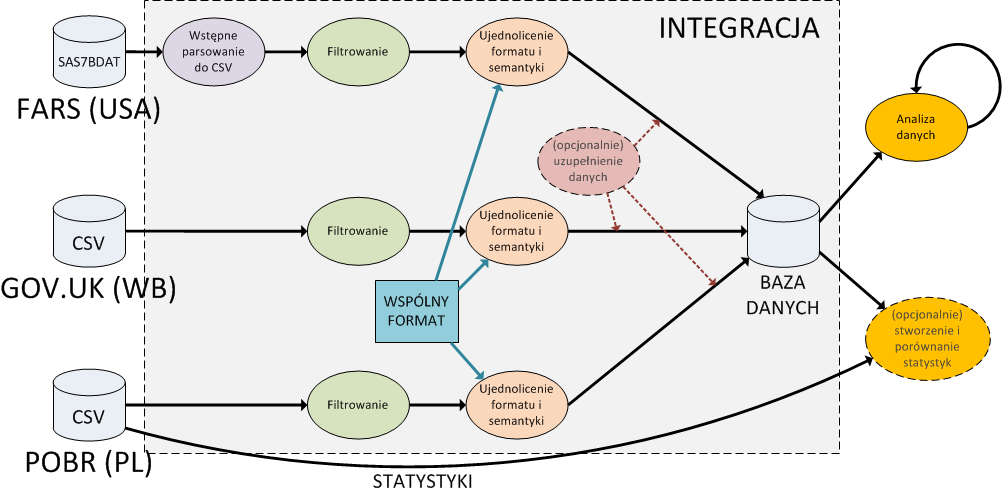
\includegraphics[width=0.9\textwidth]{images/schemat_integracji.png}}

\section{Pobranie danych}\label{pobranie-danych}

W wyniku przeprowadzonej analizy źródeł danych, której rezultaty zostały
przedstawione w dokumencie \href{Analiza-źródeł-danych}{Analiza żródeł
danych}, wytypowane zostały źródła danych, które zostaną wykorzystane w
projekcie. Pierwszą fazą realizacji projektu jest uzyskanie dostępu do
danych, oraz pobranie ich ze źródeł. Wybrane dane pochodzą z trzech
krajów.

\begin{itemize}
\itemsep-14pt\parskip0pt\parsep0pt
\item
  Polska - dane Polskiego Obserwatorium Ruchu Drogowego\\
\item
  Wielka Brytania - dane z witryny gov.pl\\
\item
  Stany Zjednoczone - dane z systemu FARS - Fatality Analysis Reporting
  System
\end{itemize}

W przypadku niektórych źródeł dane są dostępne do pobrania bezpośrednio
ze strony lub serwera ftp, bez ograniczeń dostępu, jednak w przypadku
danych z POBR konieczne jest uzyskanie dodatkowej autoryzacji w celu
skorzystania z pełnych danych, więc dla tego źródła danych konieczny
jest właśnie ten dodatkowy krok.

\section{Filtrowanie danych}\label{filtrowanie-danych}

Dane ze źródeł muszą następnie zostać odfiltrowane. Jest to umotywowane
zarówno dużą ilością danych jak i procesem preintegracji danych.
Dodatkowym ograniczeniem są podjęte przez nas decyzje projektowe
zawężające celowo zakres danych.

Filtrowanie danych będzie przebiegać na trzech płaszczyznach:

\begin{itemize}
\itemsep-14pt\parskip0pt\parsep0pt
\item
  stopień powagi wypadku: podjętą przez nas decyzją projektową chcemy
  się ograniczyć do wypadków śmiertelnych, będziemy więc gromadzić
  jedynie dane o takich wypadkach, odrzucając wypadki lekkie i poważne,
  ale bez skutków śmiertelnych\\
\item
  czas (wybrane roczniki) w celach interacyjnych: chcemy ograniczyć się
  do roczników, z których dane są dostępnych we wszystkich źródłach w
  celu lepszych możliwości porównania\\
\item
  czas (wybrane roczniki) w celach zapewnienia pełności danych: chcemy
  odrzucić dane z lat, dla których mamy ich zbyt mało - zakres atrybutów
  był zbyt wąski lub większość informacji jest niedostępna. Może być to
  szczególnie widoczne w danych starszych.
\end{itemize}

\section{Uwspólnienie formatu i semantyki danych}\label{uwspolnienie-formatu-i-semantyki-danych}

W celu analizy danych zróżnych źródeł konieczne jest ustalenie wspólnego
formatu danych. obejmuje on zarówno kwestie wspólnego formatu (np.
wspólny format daty), ale również uwspólnienie semantyki - przykładem
może byc opis warunków pogodowych: różne bazy przedstawiają te dane w
różny sposób, różną gamą możliwych wartości atrybutu, konieczne jest
ustalenie wspólnej listy wartości atrybutów, na którą następnie będzie
można zmapować atrybuty z poszczególnych źródeł.

Ważnym zadaniem tego etapu jest selekcja atrybutów, które będą dla nas
istotne w przeprowadzanych analizach, w szczególności selekcja atrybutów
pozwalających wnioskować o przyczynach wypadków - kryteria analizy.
Kryteria te możemy podzielić na następujące ogólne kategorie:

\begin{itemize}
\itemsep-14pt\parskip0pt\parsep0pt
\item
  data\\
\item
  miejsce\\
\item
  warunki pogodowe\\
\item
  warunki środowiskowe\\
\item
  dane o uczestnikach (np. młodzi / pijani kierowcy)\\
\item
  dane o pojazdach (np. rocznik, systemy bezp.)
\end{itemize}

Dokładny opis szczegółowych kryteriów analizy można znaleźć w dokumencie
\href{Kryteria-analizy}{Kryteria analizy}.

\section{Integracja}\label{integracja}

Integracja danych polegać będzie na sprowadzeniu danych do określonego
wcześniej wspólnego formatu. W tym celu konieczne będzie sparsowanie
danych przy pomocy skryptów w pythonie a następnie przetłumaczenie i
zmianę formatu na wspólny.

W miarę potrzeby i możliwości będziemy również na tym etapie uzupełniać
dane z dodatkowych źródeł - np. w razie braku danych o pogodzie dla
dużej ilości wypadków, można z innych źródeł pobrać informacje o
pogodzie w danym miejscu i czasie.

Tak przetłumaczone i uzupełnione dane zostaną zapisane do relacyjnej
bazy danych PostgreSQL, zgodnie z opracowanym schematem bazy danych,
który jest dokładnie opisany w dokumencie
\href{Projekt-bazy-danych}{Projekt bazy danych}.

\section{Analiza danych}\label{analiza-danych}

Kolejnym, kluczowym krokiem procesu jest analiza danych. Dane
zgromadzone w bazie będziemy analizować na kilka sposobów.

Pierwszym z nich jest analiza statystyczna. Przy pomocy narzędzi do
wizualizacji oraz narzędzi analizy statystycznej języka R czy platformy
Weka będziemy analizować statystyczne własności danych takie jak
korelacje czy procentowe udziały atrybutów. Głównymi atrybutami branymi
pod uwagę w tej analizie będą atrybuty wskazane w dokumencie
\href{Kryteria-analizy}{Kryteria analizy}. W ramach analizy wizualnej
będziemy rozważać wykresy generowane z danych a także nanosić dane na
mapy w celu dokonania przestrzennej analizy danych.

Z bardziej zaawansowanych metod, chcemy spróbować poddać dane
klasteryzacji w celu wskazania podobnych wypadków i podjęcia próby
wskazania dla nich wspólnych cech. Dodatkową formą analizy danych będzie
wyszukiwanie wzorców częstych - pozwoli ono wskazać często
współwystępujące okoliczności wypadków i wysnuć wnioski co do ich wpływu
na występowanie wypadków.

\section{Opcjonalne kierunki analizy}\label{opcjonalne-kierunki-analizy}

Jeżeli po wykonaniu wymienionych już analiz zostanie nam nieco czasu,
możemy podjąć się zrealizowania w projekcie opcjonalnych kierunków
analizy. Będą one polegać na stworzeniu zbiorczych statystyk z danych
przechowywanych w bazie i porównanie ich ze zbiorczymi danymi z
regionów, dla których nie mamy dostępu do szczegółowych danych z
wypadków. Chodzi tu szczególnie o dane z Polski, dla których nie mamy
pewności, że uda nam się otrzymać do nich dostęp.

\section{Używane technologie}\label{uzywane-technologie}

W projekcie będą wykorzystywane następujące narzędzia i technologie:

\begin{itemize}
\item
  python \cite{python}

  \begin{itemize}
  \itemsep-14pt\parskip0pt\parsep0pt
  \item
    skrypty filtrujące / parsujące / konwertujące\\
  \item
    parser sas7bdat - \cite{sas7bdat} \\
  \end{itemize}
\item
  PostgreSQL - \cite{postgres}

  \begin{itemize}
  \itemsep-14pt\parskip0pt\parsep0pt
  \item
    relacyjna baza danych do persystencji\\
  \end{itemize}
\item
  Narzędzia do analizy danych:

  \begin{itemize}
  \itemsep-14pt\parskip0pt\parsep0pt
  \item
    MS Excel\\
  \item
    R - \cite{r} \\
  \item
    Weka - \cite{weka} \\
  \end{itemize}
\item
  Narzędzia do wizualizacji danych

  \begin{itemize}
  \itemsep-14pt\parskip0pt\parsep0pt
  \item
    Polymaps - \cite{polymaps} \\
  \item
    Google Charts - \cite{gcharts} \\
  \item
    OpenLayers - \cite{openlayers}
  \end{itemize}
\end{itemize}

\section{Referencje}\label{referencje}

\begin{enumerate}
\itemsep-14pt\parskip0pt\parsep0pt
\item
  POBR - \cite{pobr}\\
\item
  FARS - \cite{fars}\\
\item
  Dane z Wielkiej Brytanii \cite{wb}
\end{enumerate}


\chapter{Kryteria analizy}
\label{chap:kryteria}
\section{Cel dokumentu}\label{cel-dokumentu}

Niniejszy dokument ma za zadanie sprecyzowanie kreteriów analizy
przyczyn wypadków. Prezentuje dane i atrybuty, na których skupimy się w
naszej analizie, gdyż podejrzewamy, że mogą mieć wpływ na powstawanie
wypadków drogowych

\section{Kryteria analizy}\label{kryteria-analizy}

\subsection{data}\label{data}

\begin{itemize}
\itemsep-14pt\parskip0pt\parsep0pt
\item
  \textbf{pora dnia:} Należy dokonać rozróżnienia dzień/noc oraz
  bardziej szczegółowego - rano/popołudnie/\ldots{} Przewidujemy, że noc
  może być czynnikiem powodującym zwiększenie ilości wypadków z powodu
  gorszej widoczności i gorszego stanu kierowcy(senność), z drugiej
  strony mniejsza liczba samochodów na drodze obniża ryzyko kolizji.
  Okolice godzin wieczornych mogą się również okazać okresem, gdzie
  narażenie na wystąpienie wypadku jest większe - zmrok powoduje znaczne
  pogorszenie widoczności, może również wystąpić senność a ruch nadal
  jest wzmożony.\\
\item
  \textbf{pora roku:} Można wnioskować, że większa liczba wypadków
  będzie występować w zimie, z powodu cięższych warunków
  atmosferycznych, jednakże mogą one skutkować większą ostrożnością
  ukierowców.
\end{itemize}

\subsection{miejsce}\label{miejsce}

\begin{itemize}
\itemsep-14pt\parskip0pt\parsep0pt
\item
  \textbf{umiejscowienie względem skrzyżowania:} Należy zbadać, czy
  wypadki częściej występują na skrzyżowaniach czy poza nimi oraz w
  ramach wypadków na skrzyżowaniach jaka zależność występuje od rodzaju
  skrzyżowania i konkretnego miejsca na skrzyżowaniu. Skłaniamy się do
  opinii, że więcej wypadków będzie się zdarzało na skrzyżowaniach z
  powodu podwyższonego ryzyka błędu i przecinania się dróg pojazdów.\\
\item
  \textbf{umiejscowienie względem przejścia dla pieszych:} Należy
  rozważyć jak częste są wypadki w okolicach przejścia dla pieszych.
  Podejrzewamy, iż obecność przejścia dla pieszych zwiększa wyzyko
  wypadku a w szególności wypadku śmiertelnego z powodu dodatkowego
  czynnika jakim są piesi, różnicy w prędkości oraz braku
  zabezpieczeń.\\
\item
  \textbf{współrzędne GPS:} Współrzędne mogą zostać wykorzystane do
  wizualizacji danych na mapie i przykładowo wnioskowaniu o większej
  liczbie wypadków w okolicach miast.
\end{itemize}

\subsection{warunki pogodowe}\label{warunki-pogodowe}

\begin{itemize}
\itemsep-14pt\parskip0pt\parsep0pt
\item
  \textbf{opady (deszcz, śnieg):} Obecność opadów niewątpliwie wpływa na
  pogorszenie widoczności a także warunków na drodze co może się
  przyczyniać do częstszego występowania wypadków. Z drugiej strony,
  kierowcy przejawiają tendencję do wytężonej uwagi i ostrożniejszej
  jazdy w takich warunkach.\\
\item
  \textbf{mgła:} Mgła jest czynnikiem zdecydowanie pogarszającym
  widoczność i sugerującym zwiększenie ryzyka wypadku.\\
\item
  \textbf{wiatr:} Silny wiatr może powodować zwiększenie ryzyka wypadku.
\end{itemize}

\subsection{warunki środowiskowe}\label{warunki-srodowiskowe}

\begin{itemize}
\itemsep-14pt\parskip0pt\parsep0pt
\item
  \textbf{oświetlenie:} może być kluczowym czynnikiem wpływającym na
  ilość wypadków, spodziewane jest znalezienie częstych wzorców
  zawierające niekorzystne oświetlenie i pogodę jako okoliczności
  wypadków.\\
\item
  \textbf{stan nawierzchni:} posłuży do poszukiwania korelacji z danymi
  na temat poślizgu / braku przyczepności pojazdów oraz do wnioskowania
  czy stan nawierzchnii może mieć duży wpływ na ilość wypadków\\
\item
  \textbf{rodzaj (klasa) drogi:} spodziewany jest wpływ tego czynnika na
  ilość wypadków oraz przewidywane jest znalezienie korelacji z takimi
  danymi jak prędkość poruszania i przekroczenie prędkości
\end{itemize}

\subsection{dane o uczestnikach}\label{dane-o-uczestnikach}

\begin{itemize}
\itemsep-14pt\parskip0pt\parsep0pt
\item
  \textbf{wiek kierowcy:} ta informacja może posłużyć do znalezienia
  zależności pomiędzy wiekiem kierowcy a powagą wypadku, stopniem
  przekroczenia prędkości, ilością ofiar etc.\\
\item
  \textbf{poprzednie wypadki kierowcy:} w celu zweryfikowania, czy osoby
  z historią wypadków i wykroczeń powodują więcej wypadków i czy uczą
  się na błędach\\
\item
  \textbf{stan kierowcy:} informacje w rodzaju czy kierowca był zaspany
  / zmęczony / niedołężny etc. mogą posłużyć do bezpośredniego
  wnioskowania o przyczynach wypadków\\
\item
  \textbf{alkohol:} pozwoli na zobrazowanie jak dużo i jak poważnych
  wypadków powodowanych jest przez pijanych kierowców\\
\item
  \textbf{narkotyki:} informacje te pojawiają się rzadziej niż związane
  z alkoholem, ale mogą pozwolić na podobne wnioskowanie\\
\item
  \textbf{typ uczestnika (pieszy, pasażer, \ldots{}):} pozwoli uzyskać
  statyski, między innymi jak często w wypadkach biorą udział osoby
  niezmotoryzowane, ile wśród nich jest ofiar, które siedzenia w
  samochodzie są najmniej bezpieczne\\
\item
  \textbf{użycie pasów bezpieczeństwa:} czy i jak wpływa na stopień
  obrażeń\\
\item
  \textbf{otwarcie poduszek powietrznych:} czy i jak wpływa na stopień
  obrażeń\\
\item
  \textbf{użycie kasku:} czy i jak wpływa na stopień obrażeń
\end{itemize}

\subsection{dane o pojazdach}\label{dane-o-pojazdach}

\begin{itemize}
\itemsep-14pt\parskip0pt\parsep0pt
\item
  \textbf{rok produkcji:} może pozwolić na szukanie wpływu na ilość i
  powagę wypadków, ilość ofiar\\
\item
  \textbf{marka:} do celów stastycznych, możliwe jest że posiadacze
  niektórych marek (Samochody sportowe) powodują więcej wypadków\\
\item
  \textbf{model:} do celów stastycznych, możliwe jest że posiadacze
  niektórych marek (Samochody sportowe) powodują więcej wypadków\\
\item
  \textbf{typ pojazdu (np. ciężarówka):} podobnie jak wyżej, może
  posłużyć do znalezienia prawidłowości jakie rodzaje samochodów
  częściej biorą udział w wypadkach\\
\item
  \textbf{prędkość poruszania się:} istotna informacja w kontekście
  korelacji z powagą wypadku, ilością ofiar\\
\item
  \textbf{przekroczenie prędkości:} istotna informacja w kontekście
  korelacji z powagą wypadku, ilością ofiar
\end{itemize}

\section{Hipotezy do weryfikacji}\label{hipotezy-do-weryfikacji}

W ramach analizy, chcemy nie tylko przeanalizować wpływ pojedynczych
atrybutów na występowanie wypadków, ale także zweryfikować bardziej
zaawansowane hipotezy dotyczące wpływu złożonych czynników na
bezpieczeństwo na drodze.

\subsection{Ograniczenie widoczności}\label{ograniczenie-widocznosci}

Czynniki ograniczające widoczność powinny mieć duży wpływ na wzrost
liczby wypadków. W szczególności groźne są kombinacje takich czynników,
przykładowo, niezwykle groźnymi warunkami na drodze są połączenie noc i
mgła, czy noc i mgła i deszcz. Można w tę analizę włączyć jeszcze stan
oświetlenia - brak oświetlenia na drodze może dodatkowo pogarszać
warunki.

Dodatkowo można rozważyć czy warunki ograniczenia widoczności nie
powodują większej liczby wypadków z udziałem pieszych. Piesi są najmniej
uprzywilejowanymi uczestnikami ruchu i są też w trudnych warunkach
najmniej widoczni, szczególnie w wypadku braku odblasków.

\subsection{Niesprzyjające warunki
atmosferyczne}\label{niesprzyjajace-warunki-atmosferyczne}

Deszcz lub śnieg albo ich połączenie są groźnymi warunkami do jazdy.
Dodatkowo silny wiatr może sprawić, iż kierowca ma ograniczoną kontrolę
nad samochodem. Należy jednak sprawdzić, czy fakt, że w trudnych
warunkach kierowcy jeżdżą zdecydowanie ostrożniej i nie decydują się na
brawurowe zachowania tak często jak w dobrych warunkach nie sprawia, że
wypadków tych nie jest tak dużo więcej jak można by się spodziewać.

\subsection{Złe warunki a przekraczanie
prędkości}\label{ze-warunki-a-przekraczanie-predkosci}

Interesującą analizą może być sprawdzenie jak często wypadki są
powodowane w niesprzyjających warunkach (atmosferycznych i
oświetleniowych) dodatkowo z przekroczeniem prędkości przez kierowcę.
Należy to porównać z wypadkami w warunkach sprzyjających.

\subsection{Rozkład atrybutów w różnych przedziałach
czasowych}\label{rozkad-atrybutow-w-roznych-przedziaach-czasowych}

Ciekawą analizą do wykonania wydaje się rozkład czasowy wartości
niektórych atrybutów. Rozważane przedziały czasowe mogą być różne:

\begin{itemize}
\itemsep-14pt\parskip0pt\parsep0pt
\item
  pora dnia\\
\item
  dzień tygodnia\\
\item
  pora roku\\
\item
  rozkład dzienny w ciągu roku
\end{itemize}

Porównanie można przeprowadzać między innymi pod następującymi
względami:

\begin{itemize}
\itemsep-14pt\parskip0pt\parsep0pt
\item
  procent wypadków z przekroczeniem prędkości\\
\item
  procent wypadków, gdzie kierowca miał alkohol we krwi\\
\item
  średnia liczba poszkodowanych w wypadku\\
\item
  procent wypadków z udziałem pieszych\\
\item
  liczba wypadków
\end{itemize}

Analiza taka może przynieść kilka bardzo ciekawych wniosków. Przykładowo
badanie rozkładu dziennego w ciągu roku może pozwolić wskazać święta w
trakcie których zwiększa się ilość wypadków bądź wypadków pod wpływem
alkoholu. Przewidujemy, że więcej nieostrożnych i brawurowych kierowców
(alkohol i przekraczanie prędkości) może być wieczorami czy w weekendy.
Ciekawe może być też porównanie liczby wypadków pomiędzy porami roku,
gorsze warunki zimowe powinny sprawić, ale być może jest to zrównoważone
przez wzmożoną ostrożność i ograniczenie wyjeżdżania autem do minimum.
Kryzysowe mogą się okazać np.okresy przejściowe między jesienią a zimą.

\section{Zaawansowane formy
analizy}\label{zaawansowane-formy-analizy}

W ramach projektu, chcemy zastosować także ekstrakcji wiedzy z danych,
bez stawiania wcześniejszych hipotez. Cel ten możemy osiągnąć na dwa
sposoby.

Pierwszą możliwością jest przeprowadzenie klasteryzacji danych o
wypadkach. Otrzymując wyniki takiej klasteryzacji, możemy przeanalizować
podobieństwa pomiędzy wypadkami znajdującymi się w jednym klastrze i
próbować wyciągnąć cechy reprezentatywne takich wypadków i dołączyć do
analizy liczność klastrów. Można także taką analizę przeprowadzić dla
reprezentantów klastrów. Istnieje ryzyko, że taka analiza może okazać
się zbyt skomplikowana i dać jedynie ograniczoną liczbę istotnych
wniosków.

Drugim sposobem jest przeprowadzenie na danych procesu ekstrakcji
wzorców częstych. Pozwoli to na wyłonienie wartości atrybutów często
występujących wspólnie w czasie wypadków. Może byś to źródłem niezwykle
ciekawych wniosków. Należy wziąć pod uwagę, ze taka analiza jest bardzo
intensywna obliczeniowo i może być trudna do przeprowadzenia na całości
danych, należy wtedy rozważyć możliwość przeprowadzenia kilku analiz na
podzbiorze danych i połączenie pośrednich wyników analiz w wynik
całościowy.


\chapter{Projekt bazy danych}
\label{chap:projekt-bazy}
\section{Cel dokumentu}\label{cel-dokumentu}

Niniejszy dokument przedstawia schemat bazy danych wykorzystywanej w
projekcie. Jest to jednocześnie określenie wspólnego formatu danych
wykorzystywanego w procesie integracji. Pola tabel wraz z opisem formatu
i ich dopuszczalnych wartości określają wspólny format i semantykę
danych.

\section{Schemat bazy danych}\label{schemat-bazy-danych}

\centerline{\centerline{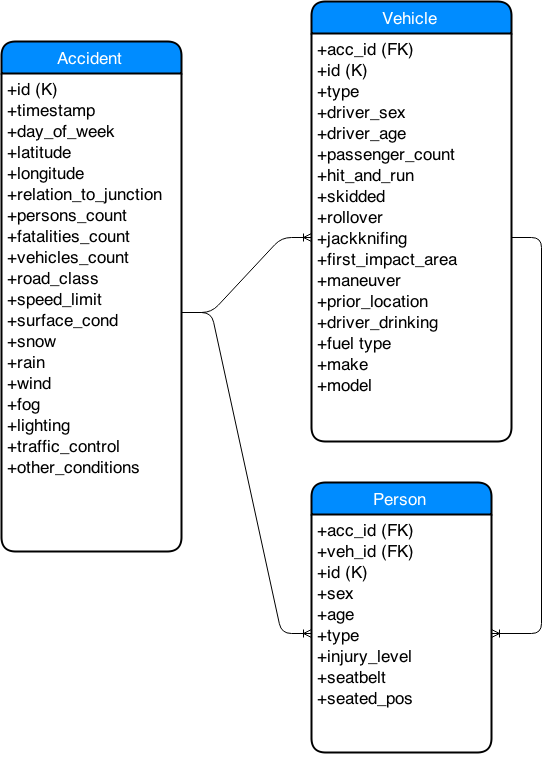
\includegraphics[scale=0.75]{images/database.png}}}

\section{Opis tabel}\label{opis-tabel}

\subsection{Accident}\label{accident}

Tabela zawierająca dane i okoliczności dotyczące wypadku

\textbf{Opis pól:}

\begin{itemize}
\item
  id - INT, klucz główny tabeli\\
\item
  timestamp - TIMESTAMP\\
\item
  day\_of\_week - INT, dzień tygodnia\\
\item
  latitude - DECIMAL, szerokość geograficzna - dla USA dane dopiero od
  1999\\
\item
  longtitude - DECIMAL, długość geograficzna - dla USA dane dopiero od
  1999\\
\item
  relation\_to\_junction - STRING

  \begin{itemize}
  \itemsep-14pt\parskip0pt\parsep0pt
  \item
    NON\_JUNCTION\\
  \item
    INTERSECTION\\
  \item
    DRIVEWAY - podjazd / prywatna droga\\
  \item
    RAMP - wjazd / zjazd z autostrady\\
  \item
    UNKNOWN\\
  \end{itemize}
\item
  persons\_count - INT, liczba uczestników w wypadku\\
\item
  fatalities\_count - INT, liczba ofiar śmiertelnych wypadku\\
\item
  vehicles\_count - INT, liczba pojazdów biorących udział w wypadku\\
\item
  road\_class - STRING, rodzaj drogi

  \begin{itemize}
  \itemsep-14pt\parskip0pt\parsep0pt
  \item
    MOTORWAY - amerykańskie Highway\\
  \item
    PRINCIPAL - brytyjska klasa A, amerykańskie Principal Arterial\\
  \item
    MAJOR - brytyjska B\\
  \item
    MINOR - brytysjka C\\
  \item
    UNCLASSIFIED\\
  \item
    UNKNOWN\\
  \end{itemize}
\item
  speed\_limit - INT, wartość ograniczenia prędkości na drodze
  {[}km/h{]}\\
\item
  surface\_cond - STRING, stan nawierzchni

  \begin{itemize}
  \itemsep-14pt\parskip0pt\parsep0pt
  \item
    DRY\\
  \item
    WET\\
  \item
    SNOW\\
  \item
    ICE\\
  \item
    FLOOD\\
  \item
    OTHER (oil, mud, sand, gravel)\\
  \item
    UNKNOWN\\
  \end{itemize}
\item
  snow - STRING, śnieg

  \begin{itemize}
  \itemsep-14pt\parskip0pt\parsep0pt
  \item
    YES - dangerous wind conditions\\
  \item
    NO\\
  \item
    UNKNOWN\\
  \end{itemize}
\item
  rain - STRING, deszcz

  \begin{itemize}
  \itemsep-14pt\parskip0pt\parsep0pt
  \item
    YES - dangerous wind conditions\\
  \item
    NO\\
  \item
    UNKNOWN\\
  \end{itemize}
\item
  wind - STRING, wiatr

  \begin{itemize}
  \itemsep-14pt\parskip0pt\parsep0pt
  \item
    YES - dangerous wind conditions\\
  \item
    NO\\
  \item
    UNKNOWN\\
  \end{itemize}
\item
  fog - mgła

  \begin{itemize}
  \itemsep-14pt\parskip0pt\parsep0pt
  \item
    YES - fog, smoke or smog\\
  \item
    NO\\
  \item
    UNKNOWN\\
  \end{itemize}
\item
  lighting - warunki oświetlenia

  \begin{itemize}
  \itemsep-14pt\parskip0pt\parsep0pt
  \item
    DAYLIGHT\\
  \item
    DARK\_LIGHTED\\
  \item
    DARK\\
  \item
    UNKNOWN\\
  \end{itemize}
\item
  traffic\_control

  \begin{itemize}
  \itemsep-14pt\parskip0pt\parsep0pt
  \item
    TRAFFIC\_SIGNAL\\
  \item
    SIGNAL\_MALF - nie działające światła\\
  \item
    STOP\_SIGN\\
  \item
    AUTH\_PERSON - osoba uprawniona do kierowania ruchem\\
  \item
    NONE - jeżeli wypadek nie na skrzyżowaniu\\
  \item
    UNKNOWN
  \end{itemize}
\end{itemize}

\subsection{Vehicle}\label{vehicle}

Tabela zawierająca dane na temat pojazdów biorących udział w wypadku i
ich kierowców. Jest powiązana relacją n:1 z tabelą \emph{Accident}
poprzez klucz obcy \emph{acc}id\_ - w jednym wypadku może brać udział
wiele pojazdów

\textbf{Opis pól:}

\begin{itemize}
\item
  acc\_id - INT, klucz obcy z tabeli \emph{Accident} realizujący relację
  1:n, wypadek w jakim brał udział dany pojazd\\
\item
  id - INT, klucz główny tabeli\\
\item
  type - STRING

  \begin{itemize}
  \itemsep-14pt\parskip0pt\parsep0pt
  \item
    CAR\\
  \item
    MOTORCYCLE\\
  \item
    BUS\\
  \item
    CARGO\\
  \item
    AGRICULTURAL\\
  \item
    OTHER\\
  \item
    UNKNOWN\\
  \end{itemize}
\item
  driver\_sex - STRING, płeć kierowcy

  \begin{itemize}
  \itemsep-14pt\parskip0pt\parsep0pt
  \item
    MALE\\
  \item
    FEMALE\\
  \item
    UNKNOWN\\
  \end{itemize}
\item
  driver\_age - INT, wiek kierowcy\\
\item
  passenger\_count - INT, liczba pasażerów\\
\item
  hit\_and\_run - STRING, czy kierujący pojazdem uciekł z miejsca
  wypadku

  \begin{itemize}
  \itemsep-14pt\parskip0pt\parsep0pt
  \item
    YES\\
  \item
    NO\\
  \item
    UNKNOWN\\
  \end{itemize}
\item
  skidded - STRING, okoliczności dotyczące poślizgu - dla USA dane te
  występują tylko w latach 2010 - 2013.

  \begin{itemize}
  \itemsep-14pt\parskip0pt\parsep0pt
  \item
    YES\\
  \item
    NO\\
  \item
    UNKNOWN\\
  \end{itemize}
\item
  rollover - STRING, okoliczności dotyczące dachowania

  \begin{itemize}
  \itemsep-14pt\parskip0pt\parsep0pt
  \item
    YES\\
  \item
    NO\\
  \item
    UNKNOWN\\
  \end{itemize}
\item
  jackknifing - STRING, okoliczności dotyczące jackknifingu

  \begin{itemize}
  \itemsep-14pt\parskip0pt\parsep0pt
  \item
    YES\\
  \item
    NO\\
  \item
    UNKNOWN\\
  \end{itemize}
\item
  first\_impact\_area - STRING, pierwsze miejsce uderzenia pojazdu

  \begin{itemize}
  \itemsep-14pt\parskip0pt\parsep0pt
  \item
    FRONT\\
  \item
    BACK\\
  \item
    LEFT\_SIDE\\
  \item
    RIGHT\_SIDE\\
  \item
    NON\_COLLISION\\
  \item
    UNKNOWN\\
  \end{itemize}
\item
  maneuver - STRING - dla USA dane te występują tylko w latach 1982 -
  2008.

  \begin{itemize}
  \itemsep-14pt\parskip0pt\parsep0pt
  \item
    STRAIGHT\\
  \item
    PARKED\\
  \item
    REVERSING\\
  \item
    U\_TURN\\
  \item
    LEFT\\
  \item
    RIGHT\\
  \item
    CHANGING\_LANE\\
  \item
    OVERTAKING\\
  \item
    HELD\_UP\\
  \item
    STOPPING\\
  \item
    STARTING\\
  \item
    CURVING\\
  \item
    UNKNOWN\\
  \end{itemize}
\item
  driver\_drinking - STRING, obecność alkoholu we krwi kierowcy

  \begin{itemize}
  \itemsep-14pt\parskip0pt\parsep0pt
  \item
    YES\\
  \item
    NO\\
  \item
    UNKNOWN\\
  \end{itemize}
\item
  fuel\_type - STRING, rodzaj paliwa - dla USA, do roku 2009, te dane
  zbierane były tylko dla ciężarówek.

  \begin{itemize}
  \itemsep-14pt\parskip0pt\parsep0pt
  \item
    DIESEL\\
  \item
    PETROL\\
  \item
    HYBRID\\
  \item
    GAS\\
  \item
    OTHER\\
  \item
    UNKNOWN
  \end{itemize}
\end{itemize}

\subsection{Person}\label{person}

Tabela zawierająca dane na temat uczestników wypadku. Powiązana relacją
n:1 z tabelą \emph{Accident} poprzez klucz obcy \emph{acc}id\_ - w
jednym wypadku może być wiele ofiar. Powiązana relacją n:1..0 z tabelą
\emph{Vehicle} poprzez klucz obcy \emph{veh}id\_ - w jednym pojeździe
może się znajdować wielu uczestników, uczestnik może się znajdować w
jednym pojeździe, lub być pieszym i nie znajdować się w żadnym
pojeździe.

\textbf{Opis pól:}

\begin{itemize}
\item
  acc\_idd - INT, klucz obcy z tabeli \emph{Accident} realizujący
  relację 1:n, wypadek w jakim brał udział dany uczestnik\\
\item
  veh\_id - INT, klucz obcy z tabeli \emph{Vehicle} realizujący relację
  0..1:n, wypadek w jakim brał udział dany uczestnik. Może zawierać
  wartość NULL.\\
\item
  id - INT, klucz główny tabeli\\
\item
  sex - STRING, płeć

  \begin{itemize}
  \itemsep-14pt\parskip0pt\parsep0pt
  \item
    MALE\\
  \item
    FEMALE\\
  \item
    UNKNOWN\\
  \end{itemize}
\item
  age - INT, wiek\\
\item
  type - STRING

  \begin{itemize}
  \itemsep-14pt\parskip0pt\parsep0pt
  \item
    DRIVER\\
  \item
    PASSENGER\\
  \item
    PEDESTRIAN\\
  \item
    UNKNOWN\\
  \end{itemize}
\item
  injury\_level - STRING, powaga obrażeń

  \begin{itemize}
  \itemsep-14pt\parskip0pt\parsep0pt
  \item
    FATAL\\
  \item
    SERIOUS\\
  \item
    SLIGHT\\
  \item
    NONE\\
  \item
    UNKNOWN\\
  \end{itemize}
\item
  seatbelt - STRING, użycie pasów bezpieczeństwa

  \begin{itemize}
  \itemsep-14pt\parskip0pt\parsep0pt
  \item
    NOT\_APPLICABLE\\
  \item
    WORN\_CONFIRMED\\
  \item
    WORN\_NOT\_CONFIRMED\\
  \item
    NOT\_WORN\\
  \item
    UNKNOWN\\
  \end{itemize}
\item
  seated\_pos - STRING, miejsce siedzenia w pojeździe

  \begin{itemize}
  \itemsep-14pt\parskip0pt\parsep0pt
  \item
    DRIVER\\
  \item
    PASSENGER\\
  \item
    BACK\\
  \item
    NONE\\
  \item
    UNKNOWN
  \end{itemize}
\end{itemize}


\chapter{Problemy podczas integracji}
\label{chap:problemy}
Na tej stronie zebrano opis problemów i trudności napotkanych podczas
parsowania i integrowania danych.

\begin{center}\rule{3in}{0.4pt}\end{center}

\textbf{Problem}:\\Niewielka cześć wypadków z USA nie posiada
określonego czasu wystąpienia.

\textbf{Rozwiązanie}:\\Odrzucić wypadki z brakującymi danymi, ponieważ
stanowią bardzo małą część rekordów (\textless{} 0.1\%).

\begin{center}\rule{3in}{0.4pt}\end{center}

\textbf{Problem}:\\Dane z USA publikowane są w różnych formatach w
zależności od roku wystąpienia.

\textbf{Rozwiązanie}:\\Poszukać bibliotek dla każdego używanego formatu
i użyć ich do sprowadzenia danych do jednego formatu (CSV).

\begin{center}\rule{3in}{0.4pt}\end{center}

\textbf{Problem}:\\Znaczenie wartości atrybutów w danych z USA zmienia
się w zależności od roku wystąpienia (np. wartość ``4'' w polu
``ATMOSPHERIC CONDITIONS'' znaczy ``deszcz'' w latah 1975 - 1990,
natomiast w późniejszych latach ``wiatr''). Część atrybutów przestaje
być wspierana po jakimś czasie, natomiast część pojawia się dopiero w
ostatnich latach. Ponadto, niektóry atrybuty przenoszone są pomiędzy
różnymi bazami danych.

\textbf{Rozwiązanie}:\\Zaprojektować mechanizm, który pozwoli na wygodne
mapowanie wartości atrybutów w zależności od roku wystąpienia i bazy
źródłowej. Schemat mapowania mógłby być zapisywany w pliku, co pozwoli
na łatwe parsowanie wszystkich danych po stworzeniu odpowiednich
schematów.

\begin{center}\rule{3in}{0.4pt}\end{center}

\textbf{Problem}:\\Bardzo duża ilość danych w zestawach z USA i GB.

\textbf{Rozwiązanie}:\\Umieścić w bazie część danych z możliwie
największym przekrojem jeśli chodzi o czas wystąpienia wypadku. W tym
celu można odrzucić część wypadków z każdego roku, ale w taki sposób,
aby uzyskać przykłady rekordów z różnych miesięcy.

\begin{center}\rule{3in}{0.4pt}\end{center}

\textbf{Problem}:\\Część rekordów posiada sporo nieokreślonych wartości
atrybutów.

\textbf{Rozwiązanie}:\\Ustalić limit nieokreślonych wartości, poniżej
którego dane będą odrzucane. Należy kierować się tym, aby zostawić
wypadki z wystarczającą do wnioskowania ilością informacji. Limit nie
może być zbyt wysoki, aby nie spowodować odrzucenia dużej części danych.

\begin{center}\rule{3in}{0.4pt}\end{center}

\textbf{Problem}:\\Część atrybutów posiada bardzo duży zakres możliwych
wartości, np. marka i model samochodu.

\textbf{Rozwiązanie}:\\Zastosować jakąś metodę przechowywania możliwych
wartości, np. w plikach tekstowych albo tabeli bazy danych, aby łatwo
było się do nich odnosić podczas parsowania danych.

\begin{center}\rule{3in}{0.4pt}\end{center}

\textbf{Problem}:\\Dane z Wielkiej Brytanii nie mają dokładnego wieku
osób, tylko zakwalifikowanie do przedziału wiekowego. Ponadto okazuje
się że może danych o wieku nie być w ogóle.

\textbf{Rozwiązanie}:\\Zastąpić przedział wiekowy reprezentatywną
wartością - np. średnią, albo losować wartość z przedziału wiekowego z
rozkładem jednostajnym. Tam gdzie wiek nie jest dostępny, zapisujemy do
bazy wiek ujemny, tak aby było wiadomo, iż brak tu danych.

\begin{center}\rule{3in}{0.4pt}\end{center}

\textbf{Problem}:\\Dane z Wielkiej Brytanii nie mają danych o wszystkich
pasażerach. Niektóre pojazdy posiadają według dostępnych danych 0
pasażerów.

\textbf{Rozwiązanie}:\\Ignorować wartość tego pola dla danych z Wielkiej
Brytanii. Niemożliwe jest uzupełnienie tych danych a szkoda stracić
wartość badawczą jaką ten atrybut daje dla danych z USA.


\chapter{Wyniki analiz}
\label{chap:wyniki-analiz}
\subsection{Cel dokumentu}\label{cel-dokumentu}

Niniejszy dokument ma na celu przestawienie wyników przeprowadzonych
analiz danych.

\subsection{Proste statystyki}\label{proste-statystyki}

Poniższa tabela przedstawia proste statystyki liczbowe dotyczące
zgromadzonych danych. Widzimy dysproporcję pomiędzy ilośćią danych
pochodzących z USA a ilością danych z Wielkiej Brytanii. Wynika z niej
podejście do analizy, w którym przeprowadzamy badania osobno na dancyh z
USA, osobno z Wielkiej Brytanii a następnie na danych połączonych.
Należy jednak mieć na uwadze, że dane połączone są mocno zdominowane
przez dane z USA.

\begin{longtable}[c]{@{}lllll@{}}
\toprule\addlinespace
Ilość danych & Wypadki & Pojazdy & Uczestniczący & Ofiary
\\\addlinespace
\midrule\endhead
USA & 1 300 141 & 1 947 730 & 3 430 324 & 1 450 505
\\\addlinespace
GB & 127 245 & 217 595 & 253 528 & 138 674
\\\addlinespace
\textbf{USA + GB} & \textbf{1 427 386} & \textbf{2 183 616} & \textbf{3
683 852} & \textbf{1 589 179}
\\\addlinespace
\bottomrule
\end{longtable}

\textbf{Analiza wypadków w czasie}

Dzień
tygodnia:\\\centerline{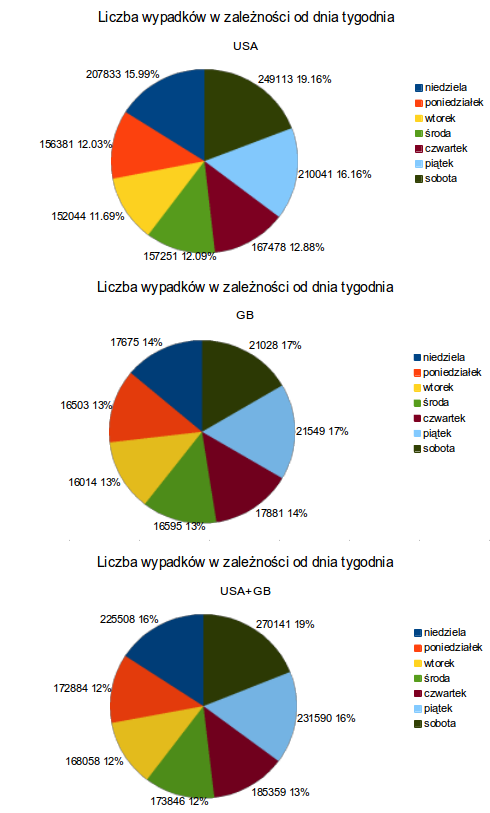
\includegraphics[width=0.8\textwidth]{images/statistics/day_of_week.png}}

Rok:\\\centerline{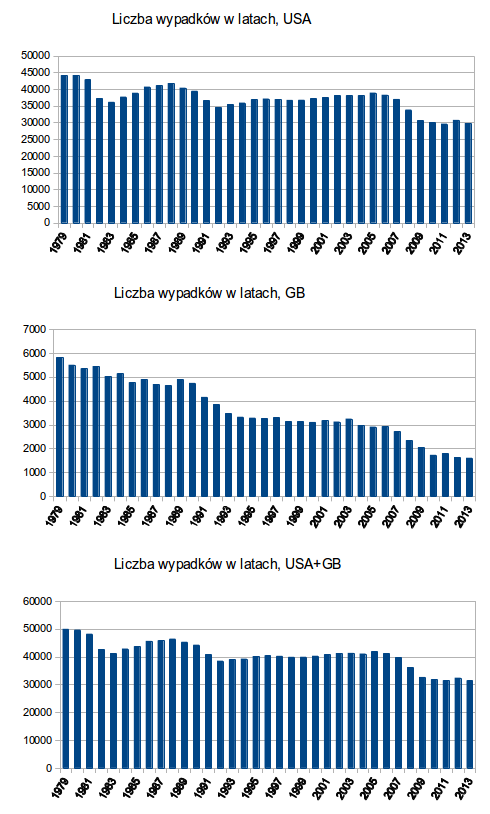
\includegraphics[width=0.8\textwidth]{images/statistics/year.png}}

Miesiąc:\\\centerline{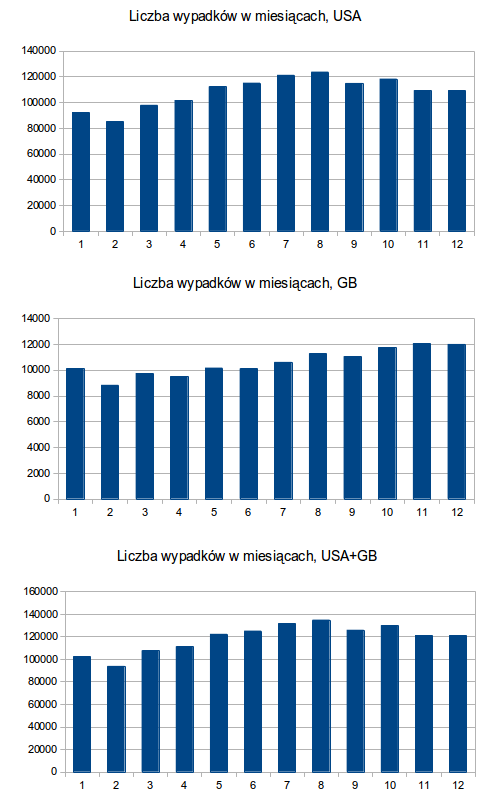
\includegraphics[width=0.8\textwidth]{images/statistics/month.png}}

Dzień:\\\centerline{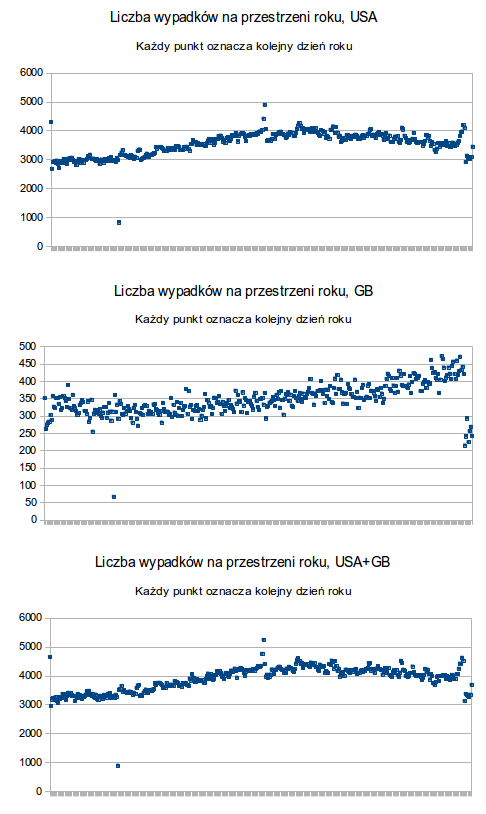
\includegraphics[width=0.8\textwidth]{images/statistics/day_of_year.png}}

Bardzo niska wartość jest dla 29.02 - występuje tylko w latach
przestępnych i istotnie jest to wartość średnio 4 razy mniejsza.

Lokalne ``piki'' - \textbf{USA}:

\begin{itemize}
\itemsep-14pt\parskip0pt\parsep0pt
\item
  01.01\\
\item
  03.07\\
\item
  04.07\\
\item
  02.08\\
\item
  03.08\\
\item
  31.10\\
\item
  01.11\\
\item
  20.12\\
\item
  21.12\\
\item
  22.12\\
\item
  23.12\\
\item
  24.12\\
\item
  31.12
\end{itemize}

Lokalne ``piki'' - \textbf{GB}:

\begin{itemize}
\itemsep-14pt\parskip0pt\parsep0pt
\item
  21.01\\
\item
  01.03\\
\item
  18.04\\
\item
  01.05\\
\item
  15.08\\
\item
  07.09\\
\item
  20.10\\
\item
  30.10\\
\item
  05.12\\
\item
  21.12
\end{itemize}

Ciekawy jest spadek liczby wypadków w ostatnich dniach roku -
spowodowany prawdopodobnie faktem, że w tym okresie znacznie mniej osób
jeździ do pracy i spędza więcej czasu w domu z rodziną.

Godzina:\\\centerline{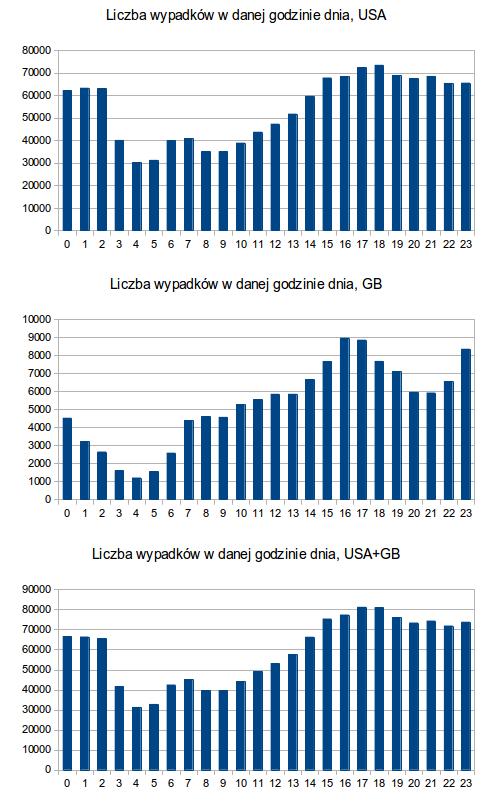
\includegraphics[width=0.8\textwidth]{images/statistics/hour.png}}

\textbf{Ograniczenie prędkości}

\centerline{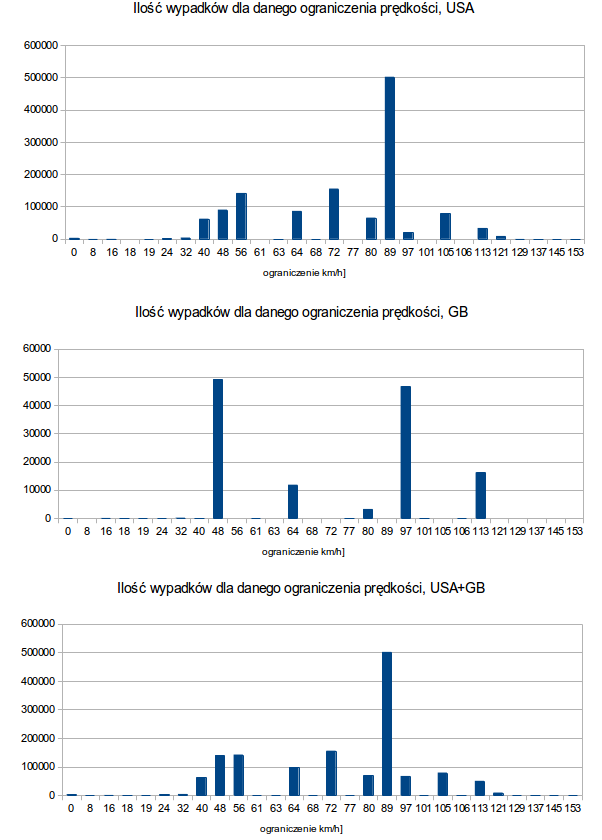
\includegraphics[width=0.8\textwidth]{images/statistics/speed_limit.png}}

\textbf{Wiek kierowcy}

\centerline{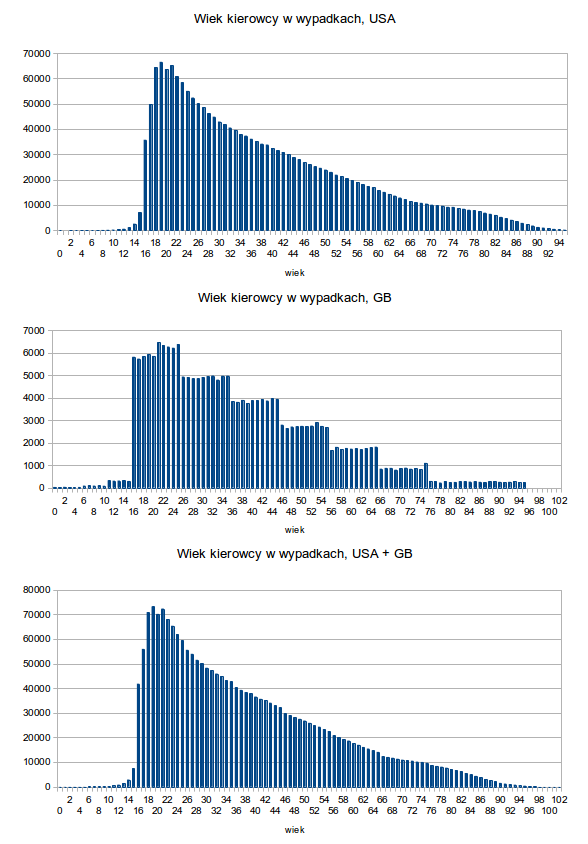
\includegraphics[width=0.8\textwidth]{images/statistics/driver_age.png}}

\textbf{Wiek uczestników wypadku}

\centerline{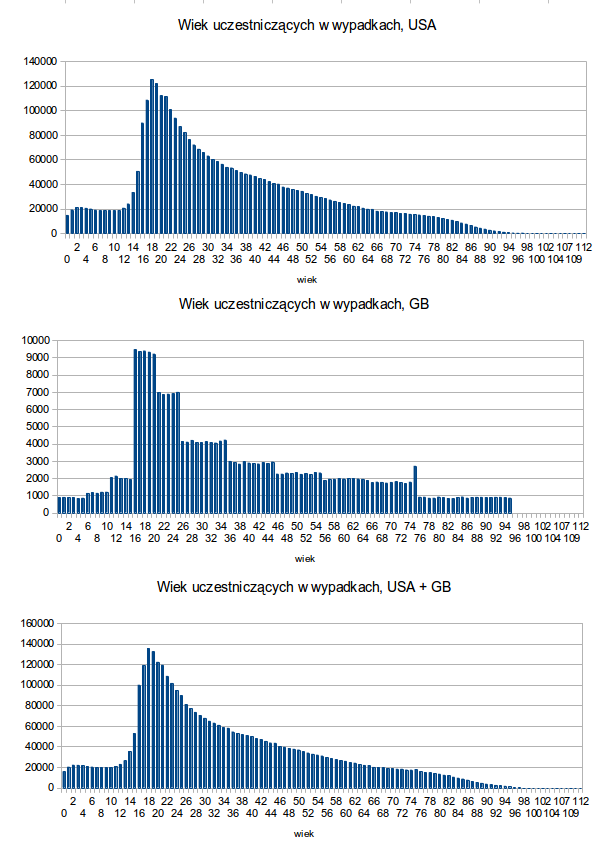
\includegraphics[width=0.8\textwidth]{images/statistics/person_age.png}}

\textbf{Kierowcy pod wpływem alkoholu}

Dane o obecności alkoholu we krwi kierowcy są dostępne jedynie dla
danych z USA.

\centerline{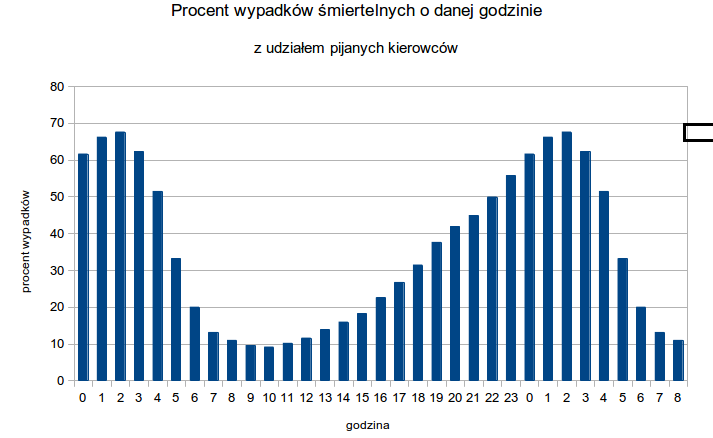
\includegraphics[width=0.8\textwidth]{images/hipotheses/drunk_drivers/hour.png}}

\centerline{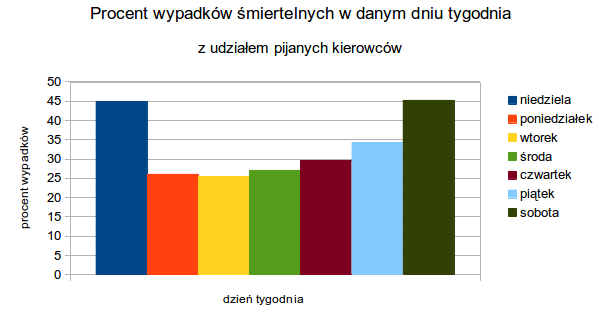
\includegraphics[width=0.8\textwidth]{images/hipotheses/drunk_drivers/day_of_week.png}}

\centerline{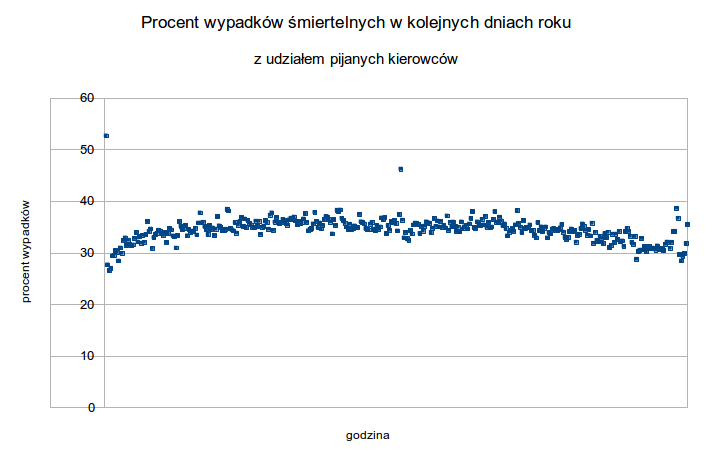
\includegraphics[width=0.8\textwidth]{images/hipotheses/drunk_drivers/day_of_year.png}}

\textbf{Warunki pogodowe}\\Udział wypadków z różnymi kombinacjami
warunków pogodowych\\S - Snow\\W - Wind\\R - Rain\\F - Fog

\begin{longtable}[c]{@{}lllllll@{}}
\toprule\addlinespace
CONDS & USA & USA \% & GB & GB \% & USA+GB & USA+GB \%
\\\addlinespace
\midrule\endhead
NONE & 1142653 & 88,17\% & 104834 & 82,98\% & 1247487 & 87,71\%
\\\addlinespace
F & 17222 & 1,33\% & 1306 & 1,03\% & 18528 & 1,30\%
\\\addlinespace
W & 445 & 0,03\% & 2798 & 2,21\% & 3243 & 0,23\%
\\\addlinespace
WF & 2 & 0,00\% & 0 & 0,00\% & 2 & 0,00\%
\\\addlinespace
R & 108652 & 8,38\% & 14463 & 11,45\% & 123115 & 8,66\%
\\\addlinespace
RF & 1444 & 0,11\% & 0 & 0,00\% & 1444 & 0,10\%
\\\addlinespace
RW & 65 & 0,01\% & 2177 & 1,72\% & 2242 & 0,16\%
\\\addlinespace
RWF & 0 & 0,00\% & 0 & 0,00\% & 0 & 0,00\%
\\\addlinespace
S & 19108 & 1,47\% & 565 & 0,45\% & 19673 & 1,38\%
\\\addlinespace
SF & 7 & 0,00\% & 0 & 0,00\% & 7 & 0,00\%
\\\addlinespace
SW & 2005 & 0,15\% & 191 & 0,15\% & 2196 & 0,15\%
\\\addlinespace
SWF & 6 & 0,00\% & 0 & 0,00\% & 6 & 0,00\%
\\\addlinespace
SR & 4283 & 0,33\% & 0 & 0,00\% & 4283 & 0,30\%
\\\addlinespace
SRF & 12 & 0,00\% & 0 & 0,00\% & 12 & 0,00\%
\\\addlinespace
SRW & 78 & 0,01\% & 0 & 0,00\% & 78 & 0,01\%
\\\addlinespace
SRWF & 0 & 0,00\% & 0 & 0,00\% & 0 & 0,00\%
\\\addlinespace
\bottomrule
\end{longtable}

\textbf{Prędkość}

\centerline{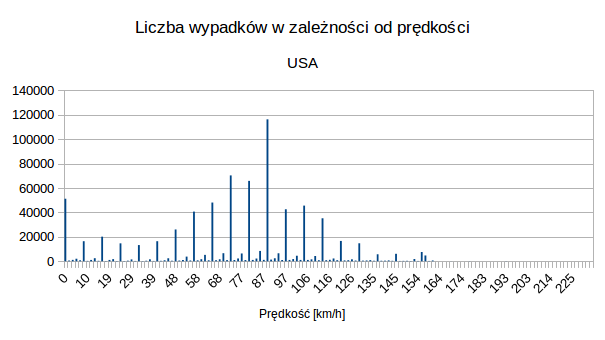
\includegraphics[width=0.8\textwidth]{images/hipotheses/speed/speed.png}}

\centerline{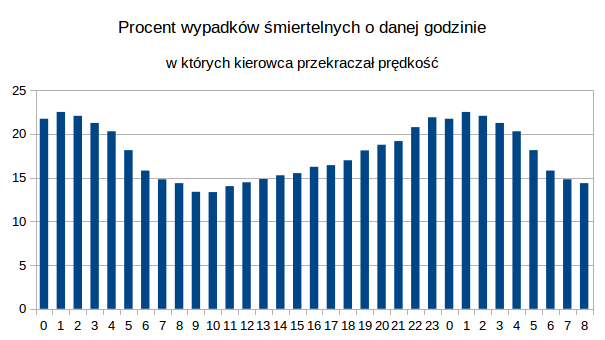
\includegraphics[width=0.8\textwidth]{images/hipotheses/speed/speed_exceeded_by_hour.png}}

\centerline{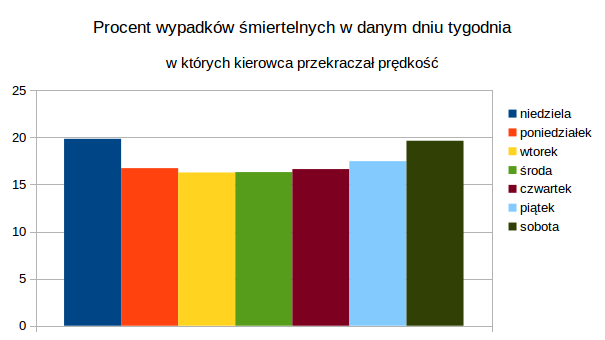
\includegraphics[width=0.8\textwidth]{images/hipotheses/speed/speed_exceeded_by_day_of_week.png}}

\centerline{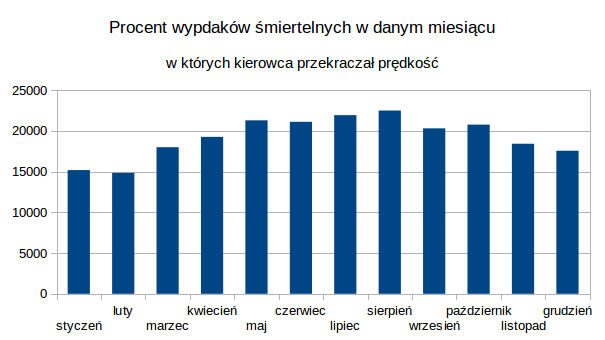
\includegraphics[width=0.8\textwidth]{images/hipotheses/speed/speed_exceeded_by_month.png}}

\centerline{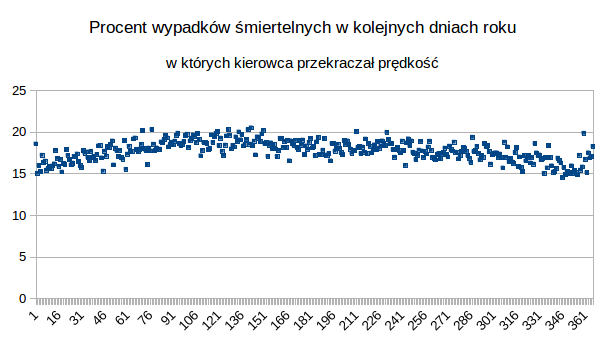
\includegraphics[width=0.8\textwidth]{images/hipotheses/speed/speed_exceeded_by_day_of_year.png}}

\centerline{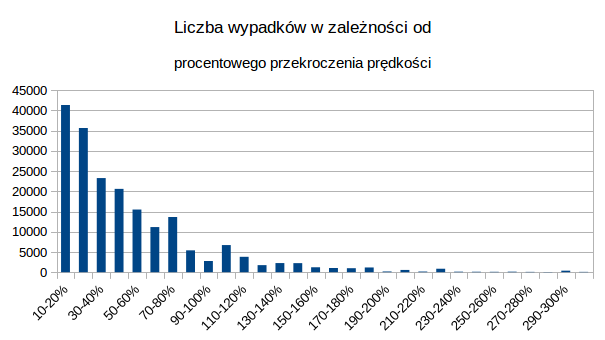
\includegraphics[width=0.8\textwidth]{images/hipotheses/speed/speed_exceeded_by_percent.png}}

\textbf{Oświetlenie}

\centerline{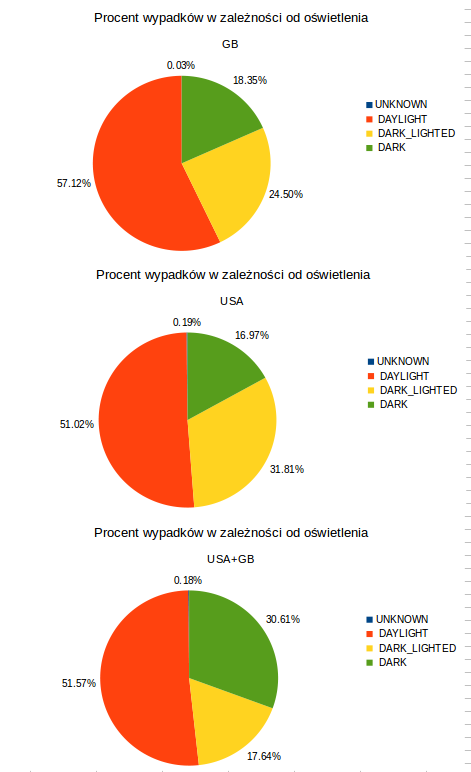
\includegraphics[width=0.8\textwidth]{images/hipotheses/lighting/lighting.png}}

\textbf{Rodzaj drogi}

\centerline{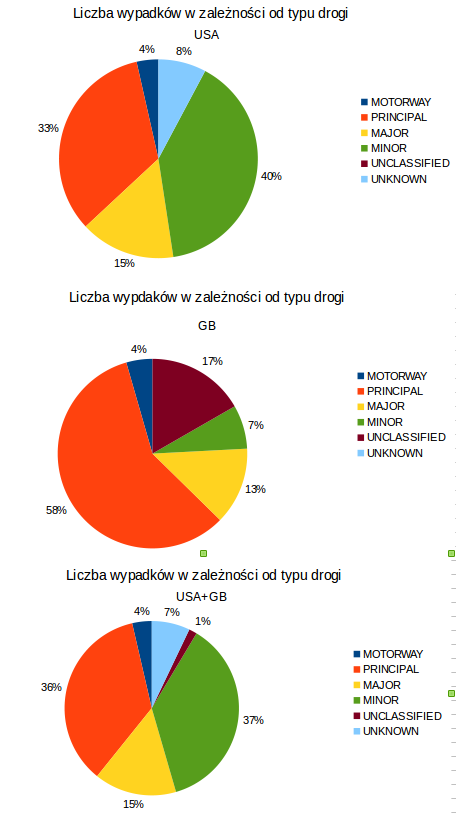
\includegraphics[width=0.8\textwidth]{images/statistics/road_type.png}}

\textbf{Piesi}

\centerline{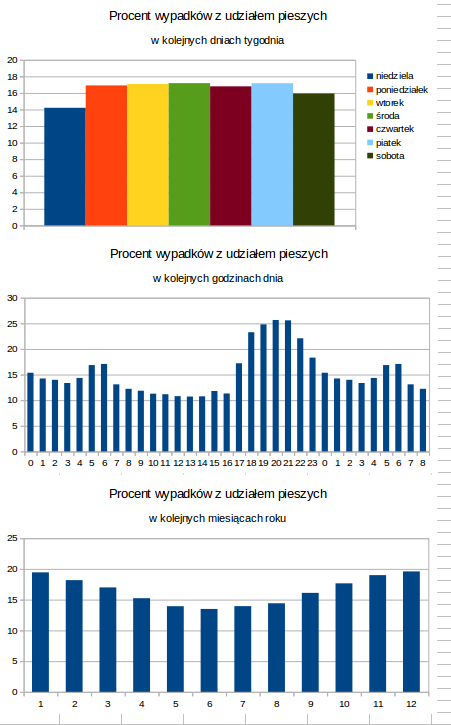
\includegraphics[width=0.8\textwidth]{images/hipotheses/pedestrians/pedestrians.png}}

Wypadki z udziałem pieszych w warunkach ograniczających widoczność.

\begin{longtable}[c]{@{}ll@{}}
\toprule\addlinespace
warunki & procent
\\\addlinespace
\midrule\endhead
wszystkie & 16.36
\\\addlinespace
deszcz & 17.10
\\\addlinespace
śnieg & 10.37
\\\addlinespace
mgła & 13.72
\\\addlinespace
ciemność & 21.51
\\\addlinespace
\bottomrule
\end{longtable}


\chapter{Hipotezy analityczne}
\label{chap:hipotezy}
\section{Cel dokumentu}\label{cel-dokumentu}

Niniejszy dokument ma na celu przedstawienie hipotez, które stawiamy
sobie w projekcie przed preprowadzeniem analizy danych. Pod kątem tych
własnie hipotez będziemy przeprowadzać analizy a następnie opisane
zostaną wyniki i wnioski wraz z komentarzem, czy hipoteza została
potwierdzona czy obalona i z czego wynika taki a nie inny rezultat.

\section{Hipotezy}\label{hipotezy}

W ramach analizy, chcemy nie tylko przeanalizować wpływ pojedynczych
atrybutów na występowanie wypadków, ale także zweryfikować bardziej
zaawansowane hipotezy dotyczące wpływu złożonych czynników na
bezpieczeństwo na drodze.

\textbf{Numer:} 1\\\textbf{Nazwa:} Ograniczenie
widoczności\\\textbf{Treść:} Czynniki ograniczające widoczność powinny
mieć duży wpływ na wzrost liczby wypadków. W szczególności groźne są
kombinacje takich czynników, przykładowo, niezwykle groźnymi warunkami
na drodze są połączenie noc i mgła, czy noc i mgła i deszcz. Można w tę
analizę włączyć jeszcze stan oświetlenia - brak oświetlenia na drodze
może dodatkowo pogarszać warunki.

\textbf{Numer:} 2\\\textbf{Nazwa:} Ograniczenie widoczności i
piesi\\\textbf{Treść:} Warunki ograniczenia widoczności mogą powodować
większą liczbę wypadków z udziałem pieszych. Piesi są najmniej
uprzywilejowanymi uczestnikami ruchu i są też w trudnych warunkach
najmniej widoczni, szczególnie w wypadku braku odblasków.

\textbf{Numer:} 3\\\textbf{Nazwa:} Niesprzyjające warunki atmosferyczne
a ostrożność kierowców\\\textbf{Treść:} Deszcz lub śnieg albo ich
połączenie są groźnymi warunkami do jazdy. Dodatkowo silny wiatr może
sprawić, iż kierowca ma ograniczoną kontrolę nad samochodem. Należy
jednak sprawdzić, czy fakt, że w trudnych warunkach kierowcy jeżdżą
zdecydowanie ostrożniej i nie decydują się na brawurowe zachowania tak
często jak w dobrych warunkach nie sprawia, że wypadków tych nie jest
tak dużo więcej jak można by się spodziewać.

\textbf{Numer:} 4\\\textbf{Nazwa:} Złe warunki a przekraczanie
prędkości\\\textbf{Treść:} W niesprzyjających warunkach (atmosferycznych
i oświetleniowych) kierowcy będą rzadziej przekraczać prędkość niż w
warunkach sprzyjających, stąd większy procent wypadków przy dodatkowym
przekroczeniu prędkości będzie w warunkach sprzyjających.

\textbf{Numer:} 5\\\textbf{Nazwa:} Alkohol we krwi kierowcy a
czas\\\textbf{Treść:} Częściej wypadki spowodowane obecnością alkoholu
we krwi kierowcy będą zdarzać się w okolicach świąt, wieczorami i w
weekendy.

\textbf{Numer:} 6\\\textbf{Nazwa:} Przekraczanie prędkości a
czas\\\textbf{Treść:} Rzadziej wypadki spowodowane przekroczeniem
prędkości przez kierowcę będą zdarzać się w zimie i na jesień niż w
pozostałych porach roku, gdyż kierowcy są ostrożniejsi w trudniejszych
warunkach.

\textbf{Numer:} 7\\\textbf{Nazwa:} Wypadki z udziałem pieszych a
czas\\\textbf{Treść:} Wypadki z udziałem pieszych mogą być częstsze w
weekendy oraz na wiosnę i w lecie, wtedy pieszych na drogach jest
więcej.

\textbf{Numer:} 8\\\textbf{Nazwa:} Liczba wypadków a
czas\\\textbf{Treść:} W ciągu dnia wypadków może być więcej w godzinach
szczytu, wieczorem w okolicach zmroku, kiedy widoczność jest najgorsza.
W ciągu roku mogłoby być ich więcej w zimie, z powodu gorszych warunków.
W skali roku na poziomie dni może ich być njawięcej w okolicach świąt,
gdyż jest wtedy wzmożony ruch i więcej pijanych kierowców (patrz
hipoteza 5).

\textbf{Numer:} 9\\\textbf{Nazwa:} Wypadki a wiek
kierowców\\\textbf{Treść:} Najwięcej wypadków będzie powodowanych przez
kierowców młodych ze względu na brawurę i brak doświadczenia.

\textbf{Numer:} 10\\\textbf{Nazwa:} Wypadki a rodzaj
drogi\\\textbf{Treść:} Na autostradach będzie mało wypadków, ponieważ są
one bezpiecznymi drogami - obowiązuje na nich nieskomplikowany sposób
poruszania się, nie ma skrzyżowań, oraz mieszkańcy USA i WB są
przyzwyczajeni do częstego korzystania z nich. Ponadto nie poruszają się
po nich piesi. Natomiast więcej wypadków może pojawić się na drogach o
randze porównywalnej z polskimi krajowymi oraz wojewódzkimi (Principal,
Major), ponieważ z jednej strony mogą mieć skomplikowana infrastrukturę
co może wymagać więcej umiejętności od kierowców, a z drugiej pozwalają
osiągnąć znaczne prędkości. Możliwe jest też zaobserwowanie znacznej
ilości wypadków śmiertelnych na drogach drugorzędnych (Minor), ponieważ
często na terenach wiejskich ludzie dopuszczają się bardziej brawurowej
jazdy i kierowania po spożyciu, gdyż rzadziej można tam spotkać
funkcjonariuszy drogówki.


\chapter{Weryfikacja hipotez}
\label{chap:weryfikacja-hipotez}

\section{Hipoteza 1}
\subsection{Opis hipotezy}\label{opis-hipotezy}

\textbf{Numer:} 1\\\textbf{Nazwa:} Ograniczenie
widoczności\\\textbf{Treść:} Czynniki ograniczające widoczność powinny
mieć duży wpływ na wzrost liczby wypadków. W szczególności groźne są
kombinacje takich czynników, przykładowo, niezwykle groźnymi warunkami
na drodze są połączenie noc i mgła, czy noc i mgła i deszcz. Można w tę
analizę włączyć jeszcze stan oświetlenia - brak oświetlenia na drodze
może dodatkowo pogarszać warunki.

\subsection{Wyniki związane z
hipotezą}\label{wyniki-zwiazane-z-hipoteza}

\textbf{Warunki pogodowe}

Udział wypadków z różnymi kombinacjami warunków pogodowych\\S - Snow\\W
- Wind\\R - Rain\\F - Fog

\begin{longtable}[c]{@{}lllllll@{}}
\toprule\addlinespace
CONDS & USA & USA \% & GB & GB \% & USA+GB & USA+GB \%
\\\addlinespace
\midrule\endhead
NONE & 1142653 & 88,17\% & 104834 & 82,98\% & 1247487 & 87,71\%
\\\addlinespace
F & 17222 & 1,33\% & 1306 & 1,03\% & 18528 & 1,30\%
\\\addlinespace
W & 445 & 0,03\% & 2798 & 2,21\% & 3243 & 0,23\%
\\\addlinespace
WF & 2 & 0,00\% & 0 & 0,00\% & 2 & 0,00\%
\\\addlinespace
R & 108652 & 8,38\% & 14463 & 11,45\% & 123115 & 8,66\%
\\\addlinespace
RF & 1444 & 0,11\% & 0 & 0,00\% & 1444 & 0,10\%
\\\addlinespace
RW & 65 & 0,01\% & 2177 & 1,72\% & 2242 & 0,16\%
\\\addlinespace
RWF & 0 & 0,00\% & 0 & 0,00\% & 0 & 0,00\%
\\\addlinespace
S & 19108 & 1,47\% & 565 & 0,45\% & 19673 & 1,38\%
\\\addlinespace
SF & 7 & 0,00\% & 0 & 0,00\% & 7 & 0,00\%
\\\addlinespace
SW & 2005 & 0,15\% & 191 & 0,15\% & 2196 & 0,15\%
\\\addlinespace
SWF & 6 & 0,00\% & 0 & 0,00\% & 6 & 0,00\%
\\\addlinespace
SR & 4283 & 0,33\% & 0 & 0,00\% & 4283 & 0,30\%
\\\addlinespace
SRF & 12 & 0,00\% & 0 & 0,00\% & 12 & 0,00\%
\\\addlinespace
SRW & 78 & 0,01\% & 0 & 0,00\% & 78 & 0,01\%
\\\addlinespace
SRWF & 0 & 0,00\% & 0 & 0,00\% & 0 & 0,00\%
\\\addlinespace
\bottomrule
\end{longtable}

\textbf{Oświetlenie}

\centerline{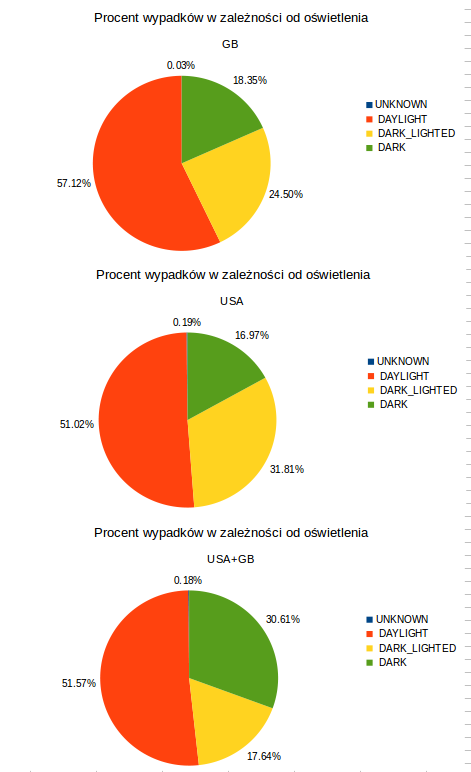
\includegraphics[width=0.8\textwidth]{images/hipotheses/lighting/lighting.png}}

\subsection{Weryfikacja i wnioski}\label{weryfikacja-i-wnioski}

Analiza tabeli dotyczącej wpływu warunków pogodowych na liczbę wypadków
pokazuje, że pod tym względem hipoteza sprawdza się w ograniczonym
zakresie, prawie 80 - 90\% wypadków występuje przy pogodzie
nieutrudniającej jazdy. Warto zauważyć wyższą wartość procentową
wypadków w trakcie deszczu dla Wielkiej Brytanii - związane jest to
zapewne z faktem, że pogoda Wielkiej Brytanii jest stosunkowo często
deszczowa.

Wydaje się, że zła pogoda podwyższa nieco liczbę wypadków. W deszczowej
Wielkiej Brytanii możemy się spodziewać, że deszcz pada przez
przynajmniej 10\% czasu. Oznacza to, że udział wypadków przy pogodzie
deszczowej jest trochę wyższy niż statystycznie uzadaniony i deszcz
przyczynia się do zwiększenia liczby wypadków. Z drugiej strony analiza
\href{Hipoteza-8}{hipotezy 8} pokazuje, że rozkład wypadków w miesiącach
różni się między USA i Wielką Brytanią. W miesiącach najbardziej
deszczowych (październik, listopad, grudzień) mamy do czynienia z
podwyższeniem liczby wypadków w Wielkiej Brytanii, w USA za to
największa jest liczba wypadków w miesiącach wakacyjnych (lipiec,
sierpień), kiedy warunki do jazdy powinny być nalepsze.

Liczba wypadków przy opadach śniegu jest procentowo większy w USA. Ma to
sens, jako że w łagodnym klimacie Wielkiej Brytanii śnieg pada niezwykle
rzadko. Wartości te sugerują, że śnieg również wpływa na zwiększenie
prawdopodobieństwa wypadków. Wartości te wydają się być wyższe niż te
statystycznie uzasadnione.

Wykresy dotyczące oświetlenia pokazują, że ciemność wpływa na wzrost
liczby wypadków. Wniosek ten płynie stąd, że niewątpliwie ruch w nocy
jest mniejszy, więc prawdopodobieństwo wypadku w nocy powinno być
znacznie mniejsze. Wykresy pokazują jednak, że prawie połowa wypadków
zdarza się w ciemności, co implikuje wzrost prawdopodobieństwa wypadku w
takich warunkach. Szczególnie widoczne jest to w Stanach Zjednoczonych,
nieco mniejszy procent w Wielkiej Brytanii.

Podsumowując, trudne warunki nie wpływają aż tak bardzo na wzrostliczby
wypadków jak można by się spodziewać. Nadal znacząca większość wypadków
zdarza się w warunkach sprzyjających. Działają tu prawdopodobnie
czynniki psychologiczne - w warunkach gorszych jesteśmy ostrożniejsi i
bardziej uważamy na to co dzieje się na drodze, niwelując niekorzystny
wpływ warunków.


\section{Hipoteza 2}
\subsection{Opis hipotezy}\label{opis-hipotezy}

\textbf{Numer:} 2\\\textbf{Nazwa:} Ograniczenie widoczności i
piesi\\\textbf{Treść:} Warunki ograniczenia widoczności mogą powodować
większą liczbę wypadków z udziałem pieszych. Piesi są najmniej
uprzywilejowanymi uczestnikami ruchu i są też w trudnych warunkach
najmniej widoczni, szczególnie w wypadku braku odblasków.

\subsection{Wyniki związane z
hipotezą}\label{wyniki-zwiazane-z-hipoteza}

\begin{longtable}[c]{@{}ll@{}}
\toprule\addlinespace
warunki & procent
\\\addlinespace
\midrule\endhead
wszystkie & 16.36
\\\addlinespace
deszcz & 17.10
\\\addlinespace
śnieg & 10.37
\\\addlinespace
mgła & 13.72
\\\addlinespace
ciemność & 21.51
\\\addlinespace
\bottomrule
\end{longtable}

\subsection{Weryfikacja i wnioski}\label{weryfikacja-i-wnioski}

Można powiedzieć iż hipoteza potwierdziła się częściowo. Widzimy wyższy
procent wypadków z pieszymi w przypadku deszczu oraz ciemności.
Szczególnie ta druga pokazuje konieczność edukowania ludzi co do
konieczności noszenia na odzieży elementów odblaskowych, aby kierowca
miał szansę zauważyć pieszego na ulicy.

Ciekawa jest dużo niższa wartość dla śniegu i mgły. Może być to związane
z wzmożoną ostrożnością kierowców w takich warunkach oraz rzadszym
wychodzeniem pieszych na drogę, szczególnie kiedy pada śnieg. W deszczu
nie obserwujemy jednak tego efektu, a piesi są mniej widoczni, stąd już
wzrost w warunkach deszczowych.


\section{Hipoteza 3}
\subsection{Opis hipotezy}\label{opis-hipotezy}

\textbf{Numer:} 3\\\textbf{Nazwa:} Niesprzyjające warunki atmosferyczne
a ostrożność kierowców\\\textbf{Treść:} Deszcz lub śnieg albo ich
połączenie są groźnymi warunkami do jazdy. Dodatkowo silny wiatr może
sprawić, iż kierowca ma ograniczoną kontrolę nad samochodem. Należy
jednak sprawdzić, czy fakt, że w trudnych warunkach kierowcy jeżdżą
zdecydowanie ostrożniej i nie decydują się na brawurowe zachowania tak
często jak w dobrych warunkach nie sprawia, że wypadków tych nie jest
tak dużo więcej jak można by się spodziewać.

\subsection{Wyniki i weryfikacja}\label{wyniki-i-weryfikacja}

Wyniki i wnioski dotyczące tej hipotezy zostały zawarte w dokumencie
dotyczącym \href{Hipoteza-1}{hipotezy 1}.


\section{Hipoteza 4}
\subsection{Opis hipotezy}\label{opis-hipotezy}

\textbf{Numer:} 4\\\textbf{Nazwa:} Złe warunki a przekraczanie
prędkości\\\textbf{Treść:} W niesprzyjających warunkach (atmosferycznych
i oświetleniowych) kierowcy będą rzadziej przekraczać prędkość niż w
warunkach sprzyjających, stąd większy procent wypadków przy dodatkowym
przekroczeniu prędkości będzie w warunkach sprzyjających.

\subsection{Wyniki związane z
hipotezą}\label{wyniki-zwiazane-z-hipoteza}

Procent wypadków, w których przekroczono prędkość w różnych warunkach

\begin{longtable}[c]{@{}ll@{}}
\toprule\addlinespace
warunki & procent
\\\addlinespace
\midrule\endhead
wszystkie & 17.79
\\\addlinespace
deszcz & 12.60
\\\addlinespace
śnieg & 6.50
\\\addlinespace
mgła & 14.76
\\\addlinespace
ciemność & 19.83
\\\addlinespace
\bottomrule
\end{longtable}

\subsection{Weryfikacja i wnioski}\label{weryfikacja-i-wnioski}

Hipoteza znajduje zdecydowane potwierdzenie w danych. Najbardziej
drastyczny (trzykrotny) spadek udziału wypadków z przekroczeniem
prędkości obserwujemy, gdy pada śnieg. Trudne warunki na drodze
wymuszają często jazdę dużo poniżej ograniczenia i powodują zwiększenie
ostrożności u kierowców.

Ciekawy jest pzrost udziału wypadków z przekroczeniem prędkości w nocy.
Jest to prawdopodobnie spowodowane faktem, że w nocy na drogach jest
pusto. Jeżeli nie ma innych czynników ograniczających widoczność,
kierowcy czują się na drodze pewniej i jadą szybciej.


\section{Hipoteza 5}
\subsection{Opis hipotezy}\label{opis-hipotezy}

\textbf{Numer:} 5\\\textbf{Nazwa:} Alkohol we krwi kierowcy a
czas\\\textbf{Treść:} Częściej wypadki spowodowane obecnością alkoholu
we krwi kierowcy będą zdarzać się w okolicach świąt, wieczorami i w
weekendy.

\subsection{Wyniki związane z
hipotezą}\label{wyniki-zwiazane-z-hipoteza}

\centerline{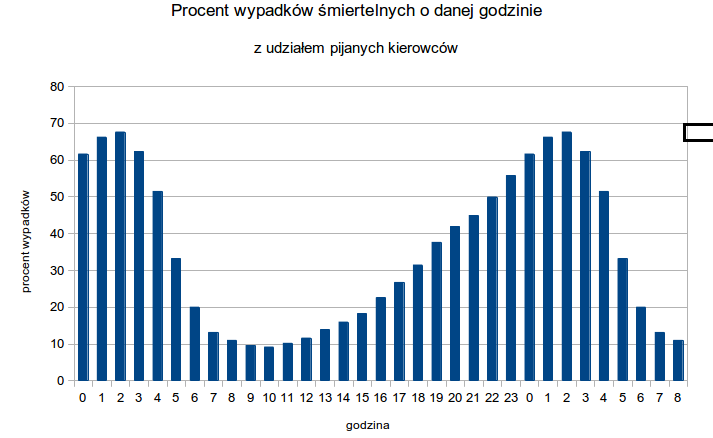
\includegraphics[width=0.8\textwidth]{images/hipotheses/drunk_drivers/hour.png}}

\centerline{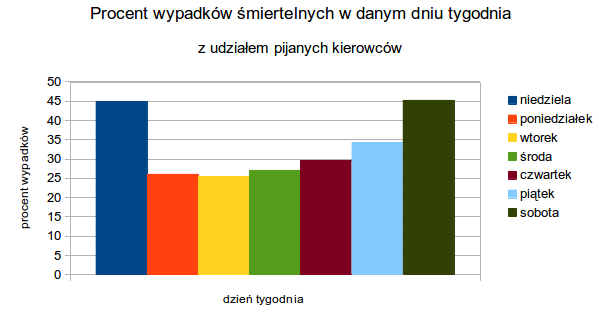
\includegraphics[width=0.8\textwidth]{images/hipotheses/drunk_drivers/day_of_week.png}}

\centerline{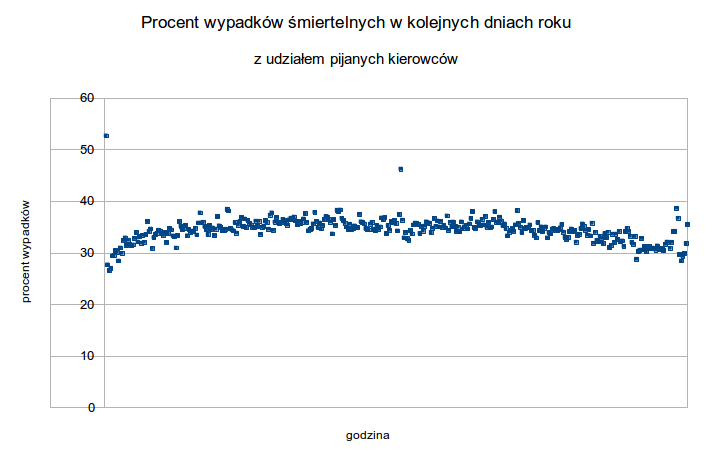
\includegraphics[width=0.8\textwidth]{images/hipotheses/drunk_drivers/day_of_year.png}}

\subsection{Weryfikacja i wnioski}\label{weryfikacja-i-wnioski}

Postawiona hipoteza sprawdziła się. Wyraźny wzrost procentowego udziału
wypadków spowodowanych przez pijanych kierowców obserwujemy w weekend -
zarówno w sobotę jak i w niedzielę jest to ok. 45\% a więc bardzo wysoka
wartość.

Patrząc na rozkład godzinny, widzimy wyraźny stały wzrost aż do godziny
2 gdzie wartość osiąga maksimum w okolicach bardzo wysokiej wartości
68\%, który następnie gwałtownie spada aż do minimum w godzinach
porannych (8 - 10).

W ciągu roku najbardziej wybija się 1 stycznia z wartością ponad 50\%
oraz święto niepodległości 4 lipca (47\%). Nieznaczny wzrost notujemy
również pod koniec roku, w okolicach świąt Bożego Narodzenia.


\section{Hipoteza 6}
\subsection{Opis hipotezy}\label{opis-hipotezy}

\textbf{Numer:} 6\\\textbf{Nazwa:} Przekraczanie prędkości a
czas\\\textbf{Treść:} Rzadziej wypadki spowodowane przekroczeniem
prędkości przez kierowcę będą zdarzać się w zimie i na jesień niż w
pozostałych porach roku, gdyż kierowcy są ostrożniejsi w trudniejszych
warunkach.

\subsection{Wyniki związane z
hipotezą}\label{wyniki-zwiazane-z-hipoteza}

\centerline{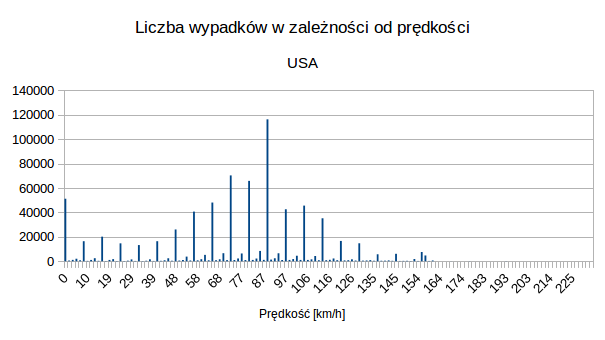
\includegraphics[width=0.8\textwidth]{images/hipotheses/speed/speed.png}}

\centerline{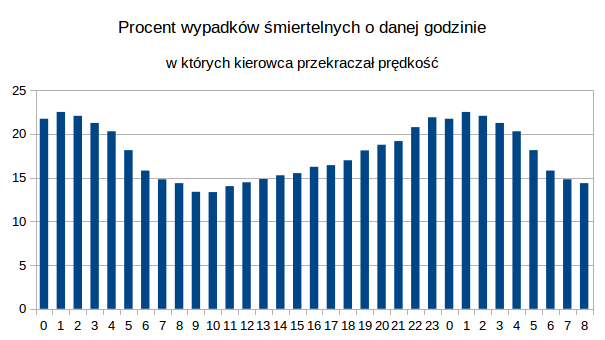
\includegraphics[width=0.8\textwidth]{images/hipotheses/speed/speed_exceeded_by_hour.png}}

\centerline{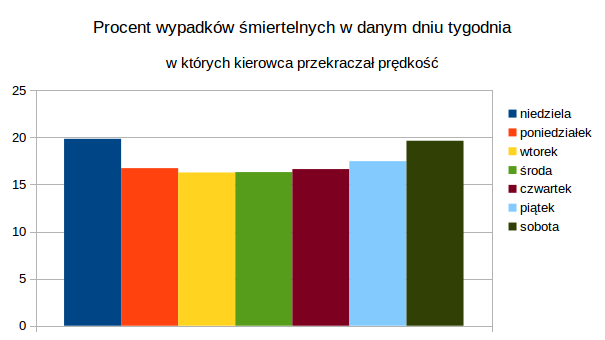
\includegraphics[width=0.8\textwidth]{images/hipotheses/speed/speed_exceeded_by_day_of_week.png}}

\centerline{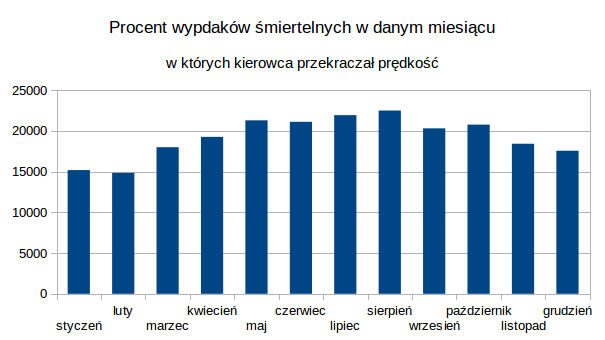
\includegraphics[width=0.8\textwidth]{images/hipotheses/speed/speed_exceeded_by_month.png}}

\centerline{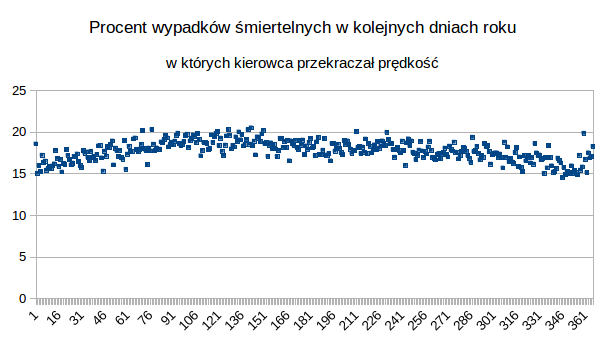
\includegraphics[width=0.8\textwidth]{images/hipotheses/speed/speed_exceeded_by_day_of_year.png}}

\subsection{Weryfikacja i wnioski}\label{weryfikacja-i-wnioski}

Hipoteza potwierdziła się. Patrząc na wykres w zależności od miesiąca
oraz dnia w roku, najmniej wypadków związanych z przekroczeniem
prędkości obserwujemy w miesiącach zimowych (styczeń, luty, grudzień).
Kierowcy z mniejszą brawurą podchodzą do jazdy w trudniejszych warunkach
i rzadziej łamią wtedy przepisy.

Większa brawura kierowców wychodzi w weekendy, wartości procentowe w
sobotę i niedzielę przekraczają o blisko 5 procent pozostałe dni.

Ciekawa jest także zależność liczby wypadków od prędkości. Widać, że
największa wartość przypada na 90 km/h.


\section{Hipoteza 7}
\subsection{Opis hipotezy}\label{opis-hipotezy}

\textbf{Numer:} 7\\\textbf{Nazwa:} Wypadki z udziałem pieszych a
czas\\\textbf{Treść:} Wypadki z udziałem pieszych mogą być częstsze w
weekendy oraz na wiosnę i w lecie, wtedy pieszych na drogach jest
więcej.

\subsection{Wyniki związane z
hipotezą}\label{wyniki-zwiazane-z-hipoteza}

\centerline{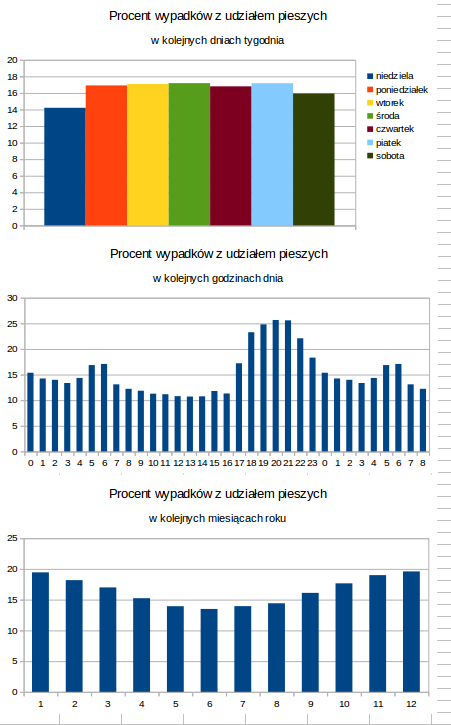
\includegraphics[width=0.8\textwidth]{images/hipotheses/pedestrians/pedestrians.png}}

\subsection{Weryfikacja i wnioski}\label{weryfikacja-i-wnioski}

Hipoteza nie potwierdziła się. Większy udział procentowy wypadków z
udziałem pieszych obserwujemy w ciągu tygodnia od poniedziałku do
piątku. W ciągu roku najmniej wypadków z udziałem pieszych jest właśnie
w miesiącach wakacyjnych (czerwiec, lipiec, sierpień).

Przyczyn takiego stanu rzeczy można szukać np. w fakcie, że jednak ruch
pieszych jest większy poza weekendem, gdyż większość ruchu pieszych to
jednak ludzie udający się do pracy/szkoły. Większy ruch pieszych
sprawia, że i wypadków z ich udziałem jest więcej.

Trudniej wytłumaczyć rozkład wypadków w ciągu roku. Można by się pokusić
o stwierdzenie, że trudniejsze warunki powodują, że wypadków z pieszymi
jest więcej i zgodnie z \href{Hipoteza-2}{hipotezą 2} czasem faktycznie
tak jest, chociaż np. śnieg sprawia, że procentowy udział wypadków z
pieszymi jest mniejszy. Można wskazać ciemność jako jeden z czynników
decydujących - w zimie czy na jesień wcześniej robi się ciemno a w
ciemności obserwujemy wyraźny wzrost procentowego udziału wypadków z
pieszymi.

Analiza wykresu godzinowego może być poparciem tezy o dużym wpływie
ruchu do/z pracy na liczbę wypadków z udziałem pieszych. Największy
procent obserwujemy w godzinach 17-22. Częściowo jest to ruch powrotny z
pracy/szkoły a później ruch związany z wieczornymi wyjściami.


\section{Hipoteza 8}
\subsection{Opis hipotezy}\label{opis-hipotezy}

\textbf{Numer:} 8\\\textbf{Nazwa:} Liczba wypadków a
czas\\\textbf{Treść:} W ciągu dnia wypadków może być więcej w godzinach
szczytu, wieczorem w okolicach zmroku, kiedy widoczność jest najgorsza.
W ciągu roku mogłoby być ich więcej w zimie, z powodu gorszych warunków.
W skali roku na poziomie dni może ich być njawięcej w okolicach świąt,
gdyż jest wtedy wzmożony ruch i więcej pijanych kierowców (patrz
\href{Hipoteza-5}{hipoteza 5}).

\subsection{Wyniki związane z
hipotezą}\label{wyniki-zwiazane-z-hipoteza}

Dzień
tygodnia:\\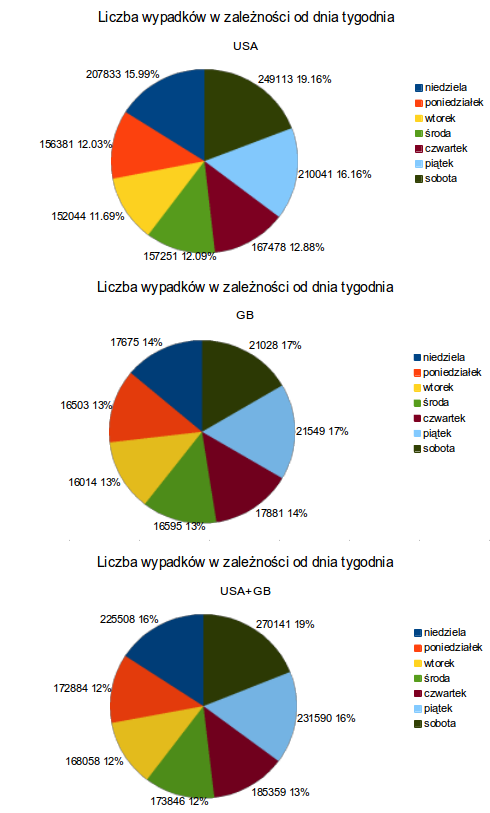
\includegraphics[width=0.8\textwidth]{images/statistics/day_of_week.png}

Rok:\\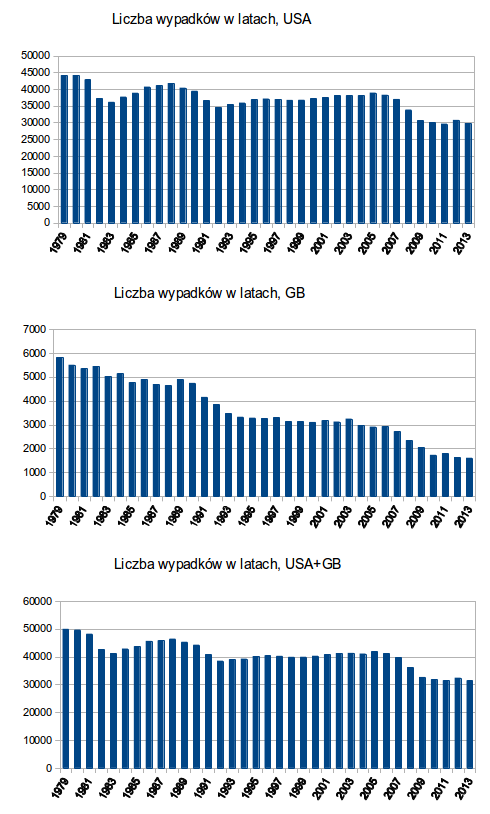
\includegraphics[width=0.8\textwidth]{images/statistics/year.png}

Miesiąc:\\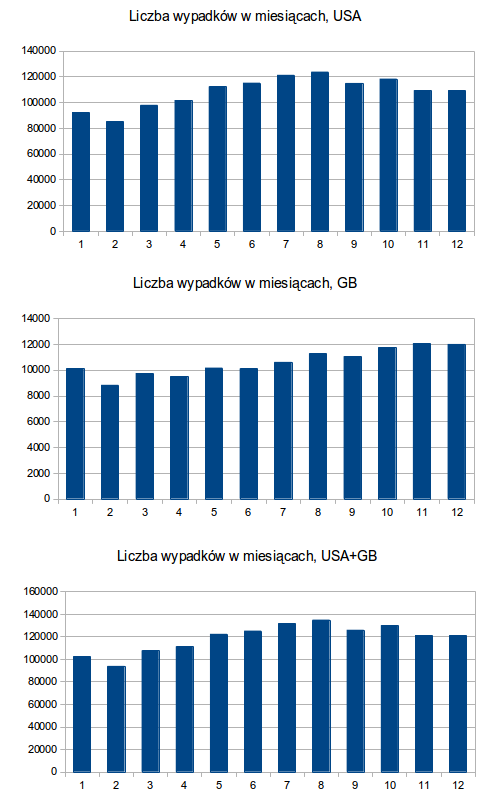
\includegraphics[width=0.8\textwidth]{images/statistics/month.png}

Dzień:\\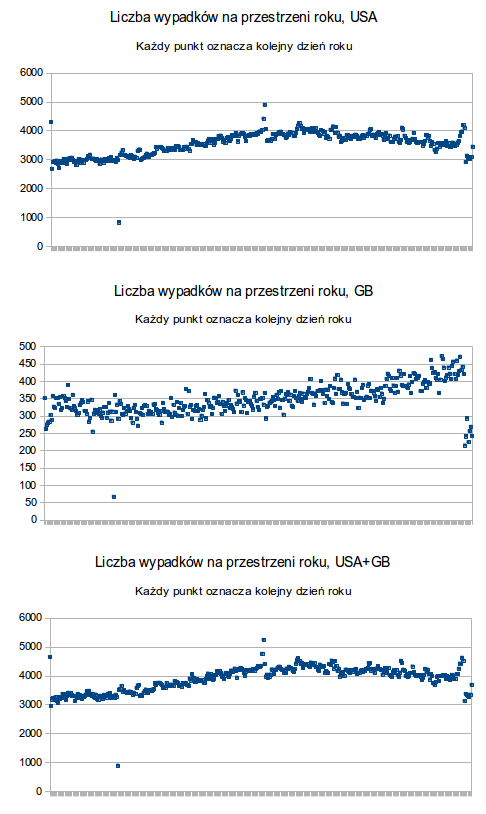
\includegraphics[width=0.8\textwidth]{images/statistics/day_of_year.png}

Bardzo niska wartość jest dla 29.02 - występuje tylko w latach
przestępnych i istotnie jest to wartość średnio 4 razy mniejsza.

Lokalne ``piki'' - \textbf{USA}:

\begin{itemize}
\itemsep1pt\parskip0pt\parsep0pt
\item
  01.01\\
\item
  03.07\\
\item
  04.07\\
\item
  02.08\\
\item
  03.08\\
\item
  31.10\\
\item
  01.11\\
\item
  20.12\\
\item
  21.12\\
\item
  22.12\\
\item
  23.12\\
\item
  24.12\\
\item
  31.12
\end{itemize}

Lokalne ``piki'' - \textbf{GB}:

\begin{itemize}
\itemsep1pt\parskip0pt\parsep0pt
\item
  21.01\\
\item
  01.03\\
\item
  18.04\\
\item
  01.05\\
\item
  15.08\\
\item
  07.09\\
\item
  20.10\\
\item
  30.10\\
\item
  05.12\\
\item
  21.12
\end{itemize}

Ciekawy jest spadek liczby wypadków w ostatnich dniach roku -
spowodowany prawdopodobnie faktem, że w tym okresie znacznie mniej osób
jeździ do pracy i spędza więcej czasu w domu z rodziną.

Godzina:\\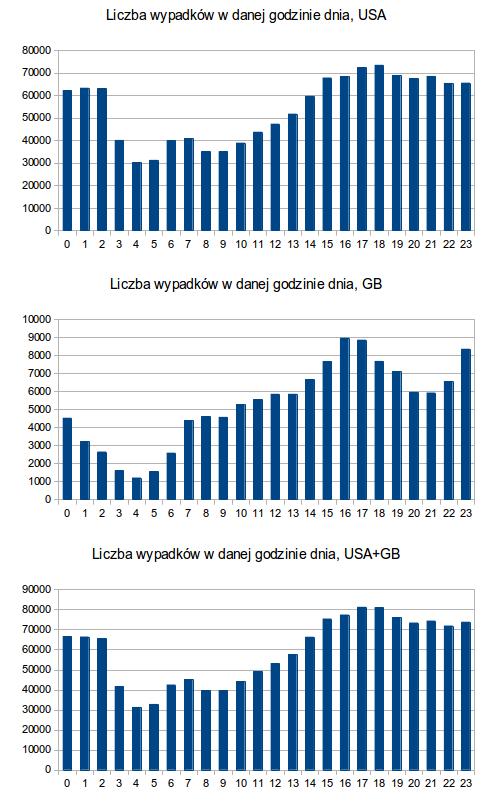
\includegraphics[width=0.8\textwidth]{images/statistics/hour.png}

\subsection{Weryfikacja i wnioski}\label{weryfikacja-i-wnioski}

Hipoteza analityczna dotycząca liczby wypadków w czasie w znacznej
mierze się potwierdziła. Podzielimy wyniki tej analizy w zależności od
rozważanych wymiarów czasowych

\subsubsection{Godzina}\label{godzina}

Bardzo wyraźnie widać wrost liczby wypadków w godzinach szczytu - w
trakcie powrotów z pracy. W Wielkiej Brytanii są to przede wszystkim
okolice godziny 16 i 17, w USA godzina 17-18. Widać również kiedy rano
ruch się zaczyna wzmagać i jest to w okolicach godziny 7, jednak nie ma
tak dużego skoku ilości wypadków dla porannej pory dojazdu do pracy.
Może to być związane z faktem że w drodze powrotnej kierowcy są bardziej
rozkojarzeni i zmęczeni niż rano. Porównanie Wielkiej Brytani i USA
pokazuje również, że w USA znacznie więcej wypadków zdarza się we
wczesnych godzinach nocnych (23 - 2). Powodem takiego stanu rzeczy może
być na przykład większy ruch tranzytowy w tych godzinach lub częstszy
wybór samochodu jako środka transportu w przypadku późnego powrotu do
domu.

\subsubsection{Miesiąc}\label{miesiac}

Analizując liczbę wypadków w kolejnych miesiącach widzimy znaczne
różnice między rozkładem w Wielkiej Brytanii i USA. W Stanach, wyraźne
nasilenie ilości wypadków jest w miesiącach wakacyjnych, mimo że można
się spodziewać, że warunki pogodowe będą wtedy lepsze. Nasilenie ruchu
musi byc znacznie większe w tym czasie, może być też większa brawura
kierowców. W Wielkiej Brytanii można bardziej wnioskować o korelacji
między warunkami pogodowymi a liczbą wypadków. Okazuje się że
najniebezpieczniejsze są październik, listopad i grudzień, kiedy warunki
nie są aż tak wymagające jak w styczniu czy w lutym, jednak ludzie nie
unikają jazdy samochodem i nie uważają tak bardzo jak w miesiącach
ściśle zimowych.

\subsubsection{Dzień tygodnia}\label{dzien-tygodnia}

Potwierdziła się hipoteza o większej liczbie wypadków w weekend. Jeżeli
dodamy wartości liczby wypadków dla piątku, soboty i niedzieli, zarówno
dla Wielkiej Brytanii jak i dla USA stanowią one około połowy całkowitej
liczby wypadków.

\subsubsection{Dzień}\label{dzien}

Z analizy rozkładu liczby wypadków na dni w ciągu roku można
zidentyfikować niektóre dni wolne. W USA wybija się 4 lipca - dzień
niepodległości. Można zauważyć wzrost np przed Halloween czy przed 6.12.
Wzrost można obserwować w okolicach Obserwujemy spadek liczby wypadków w
okresie świątecznym, kiedy ludzie mają wolne w pracy i przeważnie
spędzają ten czas w domu z rodziną.


\section{Hipoteza 9}
\subsection{Opis hipotezy}\label{opis-hipotezy}

\textbf{Numer:} 9\\\textbf{Nazwa:} Wypadki a wiek
kierowców\\\textbf{Treść:} Najwięcej wypadków będzie powodowanych przez
kierowców młodych ze względu na brawurę i brak doświadczenia.

\subsection{Wyniki związane z
hipotezą}\label{wyniki-zwiazane-z-hipoteza}

\textbf{Wiek kierowcy}

\centerline{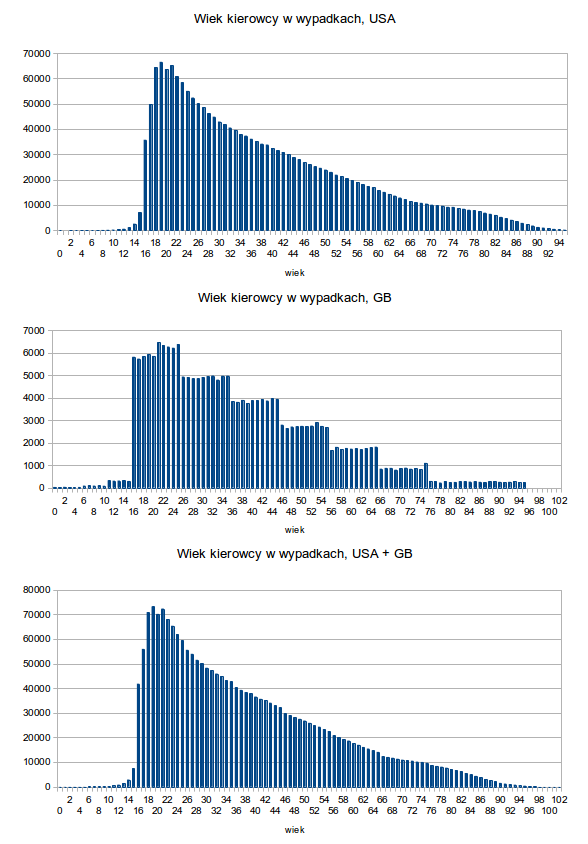
\includegraphics[width=0.9\textwidth]{images/statistics/driver_age.png}}

\textbf{Wiek uczestników wypadku}

\centerline{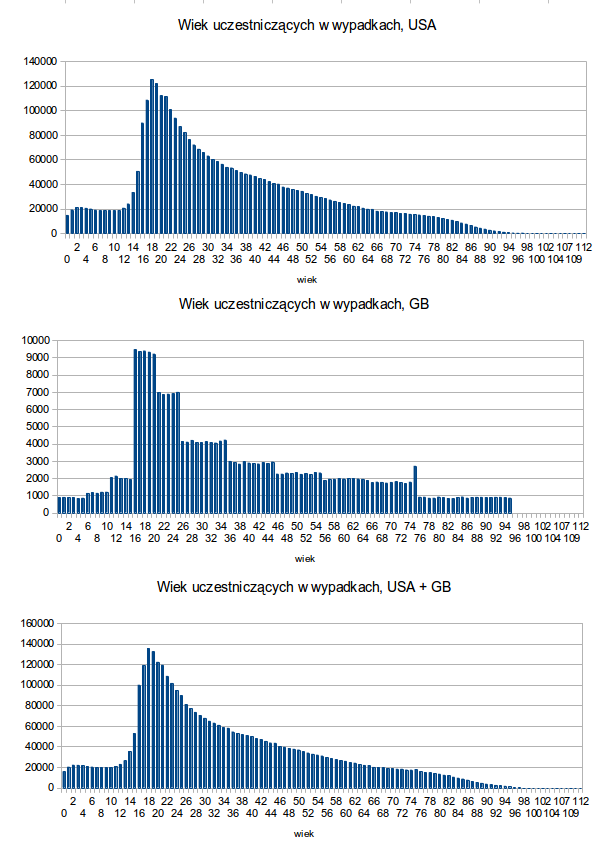
\includegraphics[width=0.9\textwidth]{images/statistics/person_age.png}}

\subsection{Weryfikacja i wnioski}\label{weryfikacja-i-wnioski}

Hipoteza potweirdziła się, największa liczba wypadków jest wśród młodych
kierowców. Jest to związane przede wszystkim z brakiem doświadczenia i
umiejętności a także często z brawurą i zbytnią pewnością siebie.

Niestety z powodu braku dokładnych danych o wieku w danych z Wielkiej
Brytanii a jedynie przedziałów wiekowych, nie widać różnicy między
wiekiem, w którym kierowcy mogą rozpocząc kierowanie pojazdami. Widać ze
w USA jest to 16 - 18 lat (zależnie od satnu), jednak dla danych z
Wielkiej Brytanii mozemy stwierdzić jedynie, że jest to gdzieś w
przedziale 16 - 21.

Analiza wieku ofiar pokazuje, poprzez swoje podobieństwo do wykresu dla
kierowców, że często kierowca jest jedyną osobą w pojeździe bądź też
podróżuje ze swoimi rówieśnikami.


\section{Hipoteza 10}
\subsection{Opis hipotezy}\label{opis-hipotezy}

\textbf{Numer:} 10\\\textbf{Nazwa:} Wypadki a rodzaj
drogi\\\textbf{Treść:} Na autostradach będzie mało wypadków, ponieważ są
one bezpiecznymi drogami - obowiązuje na nich nieskomplikowany sposób
poruszania się, nie ma skrzyżowań, oraz mieszkańcy USA i WB są
przyzwyczajeni do częstego korzystania z nich. Ponadto nie poruszają
się~po nich piesi. Natomiast więcej wypadków może pojawić się na drogach
o randze porównywalnej z polskimi krajowymi oraz wojewódzkimi
(Principal, Major), ponieważ~z jednej strony mogą mieć skomplikowana
infrastrukturę co może wymagać~więcej umiejętności od kierowców, a z
drugiej pozwalają osiągnąć znaczne prędkości. Możliwe jest też
zaobserwowanie znacznej ilości wypadków śmiertelnych na drogach
drugorzędnych (Minor), ponieważ często na terenach wiejskich ludzie
dopuszczają się bardziej brawurowej jazdy i kierowania po spożyciu, gdyż
rzadziej można tam spotkać funkcjonariuszy drogówki.

\subsection{Wyniki związane z
hipotezą}\label{wyniki-zwiazane-z-hipoteza}

\textbf{Rodzaj drogi}

\centerline{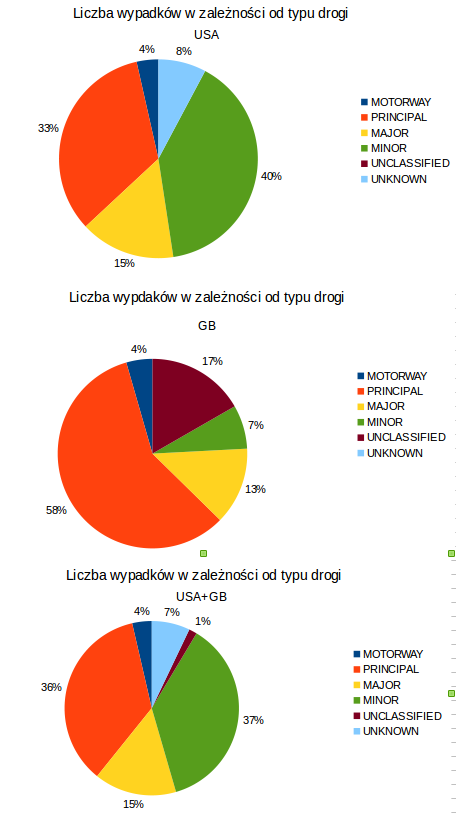
\includegraphics[width=0.8\textwidth]{images/statistics/road_type.png}}

Hipoteza potwierdziła się, na autostradach obserwuje się niewiele
wypadków śmiertelnych w porównaniu do innych typów drogi. Tutaj
instnieje spore podobieństwo pomiędzy USA a WB. Natomiast w przypadku
innych rodzajów dróg pojawiają się duże rozbieżności, choć wyniki te
potwierdzają prawdziwość hipotezy. W WB wypadki śmiertelne częściej
spotykane są na drogach krajowych, podczas gdy w USA spora część tego
udziału przypada drogom drugorzędnym. Może to wynikać z udziału
poszczególnych typów dróg w infrastrukturze danego kraju, lub
rozbieżności w ich klasyfikacjach.


\end{document}
